% Living Review research paper, generic IEEE journal draft.
% Build: pdflatex main.tex twice with shell escape disabled.
% numbers*.tex and table-*.tex come from make_tables_v3.py and analyse_real.py;
% flatten_ieee.py inlines them into a single file for Overleaf.
\documentclass[journal]{IEEEtran}
\IEEEoverridecommandlockouts

\usepackage[T1]{fontenc}
\usepackage{microtype}
\usepackage{cite}
\usepackage{amsmath,amssymb,amsfonts}
\usepackage{algorithm}
\usepackage{algpseudocode}
\usepackage{graphicx}
\usepackage{tikz}
\usetikzlibrary{arrows.meta,positioning,fit,backgrounds,calc,shapes.geometric,shapes.multipart}
\usepackage{textcomp}
\usepackage{xcolor}
\usepackage{booktabs}
\usepackage{array}
\usepackage[hyphens]{url}
\usepackage[hidelinks]{hyperref}

% outcome labels, set in sans-serif as in the original draft
\newcommand{\lbl}[1]{\textsf{#1}}
\newcommand{\qbar}{\bar{q}}
\newcommand{\sys}{Living Review}
\definecolor{ink}{HTML}{0B3C5D}
\definecolor{warn}{HTML}{B5651D}
% used by the generated tables
\newcommand{\lab}[1]{\lbl{#1}}
\newcommand{\wrong}[1]{\textcolor{warn}{\scriptsize(#1)}}
% table with a note set to the table's own width
\newsavebox{\tabbox}
\newcommand{\tablenote}[2]{\sbox{\tabbox}{#1}\usebox{\tabbox}\par\vspace{3pt}\parbox{\wd\tabbox}{\footnotesize #2}}
% Generated by make_tables_v3.py from results-v3.json; do not edit.
\newcommand{\nFiles}{117}
\newcommand{\nLines}{32,446}
\newcommand{\nPerOp}{300}
\newcommand{\nTrials}{3,600}
\newcommand{\nTrialsAll}{7,200}
\newcommand{\seedMain}{20261018}
\newcommand{\seedRep}{20261027}
\newcommand{\casCorrect}{98.5}
\newcommand{\casLo}{98.0}
\newcommand{\casHi}{98.8}
\newcommand{\casWrong}{1.5}
\newcommand{\casLost}{0.1}
\newcommand{\casRep}{98.6}
\newcommand{\casMed}{0.08}
\newcommand{\casPninetyfive}{65.1}
\newcommand{\voneCorrect}{96.4}
\newcommand{\voneLo}{95.7}
\newcommand{\voneHi}{96.9}
\newcommand{\voneWrong}{3.6}
\newcommand{\voneLost}{0.0}
\newcommand{\voneRep}{97.1}
\newcommand{\voneMed}{0.07}
\newcommand{\vonePninetyfive}{498.4}
\newcommand{\voneP}{$<10^{-16}$}
\newcommand{\voneOnlyCas}{84}
\newcommand{\voneOnlyOther}{8}
\newcommand{\qeCorrect}{74.9}
\newcommand{\qeLo}{73.4}
\newcommand{\qeHi}{76.3}
\newcommand{\qeWrong}{0.3}
\newcommand{\qeLost}{24.9}
\newcommand{\qeRep}{74.9}
\newcommand{\qeMed}{0.05}
\newcommand{\qePninetyfive}{0.2}
\newcommand{\qeP}{$<10^{-16}$}
\newcommand{\qeOnlyCas}{868}
\newcommand{\qeOnlyOther}{18}
\newcommand{\ddCorrect}{58.3}
\newcommand{\ddLo}{56.7}
\newcommand{\ddHi}{59.9}
\newcommand{\ddWrong}{0.0}
\newcommand{\ddLost}{41.7}
\newcommand{\ddRep}{58.3}
\newcommand{\ddMed}{0.26}
\newcommand{\ddPninetyfive}{1.8}
\newcommand{\ddP}{$<10^{-16}$}
\newcommand{\ddOnlyCas}{1465}
\newcommand{\ddOnlyOther}{20}
\newcommand{\lnCorrect}{41.7}
\newcommand{\lnLo}{40.1}
\newcommand{\lnHi}{43.3}
\newcommand{\lnWrong}{0.0}
\newcommand{\lnLost}{58.3}
\newcommand{\lnRep}{41.7}
\newcommand{\lnMed}{0.02}
\newcommand{\lnPninetyfive}{0.1}
\newcommand{\lnP}{$<10^{-16}$}
\newcommand{\lnOnlyCas}{2065}
\newcommand{\lnOnlyOther}{20}
\newcommand{\casSilent}{0}
\newcommand{\allSilent}{0}
\newcommand{\silentUB}{0.05}
\newcommand{\casMax}{255}
\newcommand{\recheckRecall}{99.2}
\newcommand{\falseRecheck}{0.25}
\newcommand{\nFalseRecheck}{6}
\newcommand{\nUnchanged}{2,400}
\newcommand{\nContentChanged}{1,200}
\newcommand{\nMissedRecheck}{9}
\newcommand{\missedRecheck}{0.75}
\newcommand{\recheckPrecision}{99.5}
\newcommand{\casIdentity}{100.0}
\newcommand{\casWrongIdentity}{0.0}
\newcommand{\voneIdentity}{100.0}
\newcommand{\voneWrongIdentity}{0.0}
\newcommand{\casEditElsewhere}{100.0}
\newcommand{\casWrongEditElsewhere}{0.0}
\newcommand{\voneEditElsewhere}{100.0}
\newcommand{\voneWrongEditElsewhere}{0.0}
\newcommand{\casInsertAbove}{100.0}
\newcommand{\casWrongInsertAbove}{0.0}
\newcommand{\voneInsertAbove}{100.0}
\newcommand{\voneWrongInsertAbove}{0.0}
\newcommand{\casDeleteAbove}{100.0}
\newcommand{\casWrongDeleteAbove}{0.0}
\newcommand{\voneDeleteAbove}{100.0}
\newcommand{\voneWrongDeleteAbove}{0.0}
\newcommand{\casReindent}{100.0}
\newcommand{\casWrongReindent}{0.0}
\newcommand{\voneReindent}{100.0}
\newcommand{\voneWrongReindent}{0.0}
\newcommand{\casMoveWithin}{99.0}
\newcommand{\casWrongMoveWithin}{1.0}
\newcommand{\voneMoveWithin}{99.0}
\newcommand{\voneWrongMoveWithin}{1.0}
\newcommand{\casMoveFile}{97.0}
\newcommand{\casWrongMoveFile}{3.0}
\newcommand{\voneMoveFile}{99.0}
\newcommand{\voneWrongMoveFile}{1.0}
\newcommand{\casDuplicateAbove}{100.0}
\newcommand{\casWrongDuplicateAbove}{0.0}
\newcommand{\voneDuplicateAbove}{100.0}
\newcommand{\voneWrongDuplicateAbove}{0.0}
\newcommand{\casEditToken}{95.7}
\newcommand{\casWrongEditToken}{4.3}
\newcommand{\voneEditToken}{95.0}
\newcommand{\voneWrongEditToken}{5.0}
\newcommand{\casInsertAndEdit}{96.7}
\newcommand{\casWrongInsertAndEdit}{2.7}
\newcommand{\voneInsertAndEdit}{95.0}
\newcommand{\voneWrongInsertAndEdit}{5.0}
\newcommand{\casRewrite}{97.0}
\newcommand{\casWrongRewrite}{3.0}
\newcommand{\voneRewrite}{82.0}
\newcommand{\voneWrongRewrite}{18.0}
\newcommand{\casDeleteBlock}{96.3}
\newcommand{\casWrongDeleteBlock}{3.7}
\newcommand{\voneDeleteBlock}{86.3}
\newcommand{\voneWrongDeleteBlock}{13.7}
\newcommand{\casSpanMin}{95.6}
\newcommand{\casSpanMax}{100.0}
\newcommand{\casSpanOne}{95.6}
\newcommand{\casSizeMin}{98.1}
\newcommand{\casSizeMax}{98.9}
% Generated by analyse_real.py from results-real-v1.json and results-oss-v1.json; do not edit.
\newcommand{\rN}{15,064}
\newcommand{\rPairs}{2,073}
\newcommand{\rRepos}{9}
\newcommand{\rCommits}{3,951}
\newcommand{\rExcluded}{2,205}
\newcommand{\rExcludedPct}{12.8}
\newcommand{\rUniformN}{11,449}
\newcommand{\rTargetedN}{3,615}
\newcommand{\rEditedN}{2,636}
\newcommand{\rGoneN}{144}
\newcommand{\rMovedN}{111}
\newcommand{\rShiftedN}{6,207}
\newcommand{\rInPlaceN}{5,966}
\newcommand{\rSilent}{0}
\newcommand{\rSilentAll}{1}
\newcommand{\rRecall}{98.7}
\newcommand{\rFalse}{0.00}
\newcommand{\rNFalse}{0}
\newcommand{\rNPreserved}{12,284}
\newcommand{\rNMissed}{37}
\newcommand{\rNChanged}{2,780}
\newcommand{\rNmEx}{1324}
\newcommand{\rUCas}{99.3}
\newcommand{\rUCasLo}{99.2}
\newcommand{\rUCasHi}{99.5}
\newcommand{\rUVone}{99.5}
\newcommand{\rUVoneLo}{99.4}
\newcommand{\rUVoneHi}{99.6}
\newcommand{\rUVoneD}{-0.2}
\newcommand{\rUVoneDLo}{-0.3}
\newcommand{\rUVoneDHi}{-0.1}
\newcommand{\rUVoneLead}{0.2}
\newcommand{\rUVoneLeadLo}{0.1}
\newcommand{\rUVoneLeadHi}{0.3}
\newcommand{\rUQe}{98.2}
\newcommand{\rUQeLo}{97.9}
\newcommand{\rUQeHi}{98.5}
\newcommand{\rUQeD}{1.2}
\newcommand{\rUQeDLo}{0.9}
\newcommand{\rUQeDHi}{1.4}
\newcommand{\rUQeLead}{-1.2}
\newcommand{\rUQeLeadLo}{-1.4}
\newcommand{\rUQeLeadHi}{-0.9}
\newcommand{\rUDd}{98.1}
\newcommand{\rUDdLo}{97.8}
\newcommand{\rUDdHi}{98.4}
\newcommand{\rUDdD}{1.2}
\newcommand{\rUDdDLo}{1.0}
\newcommand{\rUDdDHi}{1.5}
\newcommand{\rUDdLead}{-1.2}
\newcommand{\rUDdLeadLo}{-1.5}
\newcommand{\rUDdLeadHi}{-1.0}
\newcommand{\rULn}{49.4}
\newcommand{\rULnLo}{47.9}
\newcommand{\rULnHi}{50.8}
\newcommand{\rULnD}{50.0}
\newcommand{\rULnDLo}{48.6}
\newcommand{\rULnDHi}{51.3}
\newcommand{\rULnLead}{-50.0}
\newcommand{\rULnLeadLo}{-51.3}
\newcommand{\rULnLeadHi}{-48.6}
\newcommand{\rTCas}{67.8}
\newcommand{\rTCasLo}{66.1}
\newcommand{\rTCasHi}{69.7}
\newcommand{\rTVone}{74.6}
\newcommand{\rTVoneLo}{73.0}
\newcommand{\rTVoneHi}{76.3}
\newcommand{\rTVoneD}{-6.8}
\newcommand{\rTVoneDLo}{-8.0}
\newcommand{\rTVoneDHi}{-5.6}
\newcommand{\rTVoneLead}{6.8}
\newcommand{\rTVoneLeadLo}{5.6}
\newcommand{\rTVoneLeadHi}{8.0}
\newcommand{\rTQe}{30.2}
\newcommand{\rTQeLo}{28.2}
\newcommand{\rTQeHi}{32.2}
\newcommand{\rTQeD}{37.7}
\newcommand{\rTQeDLo}{35.5}
\newcommand{\rTQeDHi}{39.8}
\newcommand{\rTQeLead}{-37.7}
\newcommand{\rTQeLeadLo}{-39.8}
\newcommand{\rTQeLeadHi}{-35.5}
\newcommand{\rTDd}{28.5}
\newcommand{\rTDdLo}{26.6}
\newcommand{\rTDdHi}{30.4}
\newcommand{\rTDdD}{39.4}
\newcommand{\rTDdDLo}{37.2}
\newcommand{\rTDdDHi}{41.6}
\newcommand{\rTDdLead}{-39.4}
\newcommand{\rTDdLeadLo}{-41.6}
\newcommand{\rTDdLeadHi}{-37.2}
\newcommand{\rTLn}{13.2}
\newcommand{\rTLnLo}{12.0}
\newcommand{\rTLnHi}{14.5}
\newcommand{\rTLnD}{54.6}
\newcommand{\rTLnDLo}{52.7}
\newcommand{\rTLnDHi}{56.7}
\newcommand{\rTLnLead}{-54.6}
\newcommand{\rTLnLeadLo}{-56.7}
\newcommand{\rTLnLeadHi}{-52.7}
\newcommand{\rOwnN}{3,805}
\newcommand{\rOwnPairs}{457}
\newcommand{\rOwnCommits}{795}
\newcommand{\rOwnAuthors}{9}
\newcommand{\rOwnSilent}{0}
\newcommand{\rOwnUCas}{99.1}
\newcommand{\rOwnUCasLo}{98.7}
\newcommand{\rOwnUCasHi}{99.5}
\newcommand{\rOwnUVone}{99.3}
\newcommand{\rOwnUVoneLo}{98.9}
\newcommand{\rOwnUVoneHi}{99.6}
\newcommand{\rOwnUQe}{98.1}
\newcommand{\rOwnUQeLo}{97.3}
\newcommand{\rOwnUQeHi}{98.7}
\newcommand{\rOwnUDd}{98.0}
\newcommand{\rOwnUDdLo}{97.3}
\newcommand{\rOwnUDdHi}{98.7}
\newcommand{\rOwnULn}{36.4}
\newcommand{\rOwnULnLo}{33.8}
\newcommand{\rOwnULnHi}{38.9}
\newcommand{\rOwnTCas}{70.0}
\newcommand{\rOwnTCasLo}{67.0}
\newcommand{\rOwnTCasHi}{73.0}
\newcommand{\rOwnTVone}{75.4}
\newcommand{\rOwnTVoneLo}{72.4}
\newcommand{\rOwnTVoneHi}{77.9}
\newcommand{\rOwnTQe}{45.7}
\newcommand{\rOwnTQeLo}{42.1}
\newcommand{\rOwnTQeHi}{49.3}
\newcommand{\rOwnTDd}{43.8}
\newcommand{\rOwnTDdLo}{40.4}
\newcommand{\rOwnTDdHi}{47.3}
\newcommand{\rOwnTLn}{16.8}
\newcommand{\rOwnTLnLo}{14.5}
\newcommand{\rOwnTLnHi}{19.2}
\newcommand{\rOwnEditedCas}{44.0}
\newcommand{\rOwnRecall}{97.5}
\newcommand{\rOssN}{11,259}
\newcommand{\rOssPairs}{1,616}
\newcommand{\rOssCommits}{3,156}
\newcommand{\rOssAuthors}{1,036}
\newcommand{\rOssSilent}{0}
\newcommand{\rOssUCas}{99.4}
\newcommand{\rOssUCasLo}{99.2}
\newcommand{\rOssUCasHi}{99.6}
\newcommand{\rOssUVone}{99.6}
\newcommand{\rOssUVoneLo}{99.4}
\newcommand{\rOssUVoneHi}{99.7}
\newcommand{\rOssUQe}{98.2}
\newcommand{\rOssUQeLo}{97.9}
\newcommand{\rOssUQeHi}{98.5}
\newcommand{\rOssUDd}{98.1}
\newcommand{\rOssUDdLo}{97.7}
\newcommand{\rOssUDdHi}{98.4}
\newcommand{\rOssULn}{53.3}
\newcommand{\rOssULnLo}{51.6}
\newcommand{\rOssULnHi}{54.8}
\newcommand{\rOssTCas}{66.8}
\newcommand{\rOssTCasLo}{64.6}
\newcommand{\rOssTCasHi}{69.1}
\newcommand{\rOssTVone}{74.3}
\newcommand{\rOssTVoneLo}{72.3}
\newcommand{\rOssTVoneHi}{76.3}
\newcommand{\rOssTQe}{22.8}
\newcommand{\rOssTQeLo}{20.9}
\newcommand{\rOssTQeHi}{24.9}
\newcommand{\rOssTDd}{21.2}
\newcommand{\rOssTDdLo}{19.3}
\newcommand{\rOssTDdHi}{23.2}
\newcommand{\rOssTLn}{11.5}
\newcommand{\rOssTLnLo}{10.1}
\newcommand{\rOssTLnHi}{13.0}
\newcommand{\rOssEditedCas}{56.8}
\newcommand{\rOssRecall}{99.0}
\newcommand{\rPreservedMissCas}{3}
\newcommand{\rTCasHOne}{68.1}
\newcommand{\rTCasHTen}{67.4}
\newcommand{\rClsInPlaceCas}{100.0}
\newcommand{\rClsInPlaceVone}{100.0}
\newcommand{\rClsInPlaceQe}{100.0}
\newcommand{\rClsInPlaceDd}{99.9}
\newcommand{\rClsInPlaceLn}{100.0}
\newcommand{\rClsShiftedCas}{100.0}
\newcommand{\rClsShiftedVone}{100.0}
\newcommand{\rClsShiftedQe}{100.0}
\newcommand{\rClsShiftedDd}{98.7}
\newcommand{\rClsShiftedLn}{0.0}
\newcommand{\rClsMovedFileCas}{97.3}
\newcommand{\rClsMovedFileVone}{97.3}
\newcommand{\rClsMovedFileQe}{21.6}
\newcommand{\rClsMovedFileDd}{21.6}
\newcommand{\rClsMovedFileLn}{18.0}
\newcommand{\rClsEditedCas}{53.6}
\newcommand{\rClsEditedVone}{64.8}
\newcommand{\rClsEditedQe}{0.0}
\newcommand{\rClsEditedDd}{0.0}
\newcommand{\rClsEditedLn}{0.0}
\newcommand{\rClsGoneCas}{92.4}
\newcommand{\rClsGoneVone}{71.5}
\newcommand{\rClsGoneQe}{95.1}
\newcommand{\rClsGoneDd}{100.0}
\newcommand{\rClsGoneLn}{100.0}
\newcommand{\rThetaEdFifty}{76.6}
\newcommand{\rThetaGoneFifty}{61.8}
\newcommand{\rThetaEdSixty}{75.4}
\newcommand{\rThetaGoneSixty}{74.3}
\newcommand{\rThetaEdSeventy}{70.9}
\newcommand{\rThetaGoneSeventy}{81.9}
\newcommand{\rThetaEdSeventyFive}{67.4}
\newcommand{\rThetaGoneSeventyFive}{84.0}
\newcommand{\rThetaEdEighty}{62.3}
\newcommand{\rThetaGoneEighty}{88.2}
\newcommand{\rThetaEdEightyFive}{53.6}
\newcommand{\rThetaGoneEightyFive}{92.4}
\newcommand{\rThetaEdNinety}{42.6}
\newcommand{\rThetaGoneNinety}{93.8}
\newcommand{\rThetaEdNinetyFive}{26.5}
\newcommand{\rThetaGoneNinetyFive}{94.4}
\newcommand{\rCalTheta}{0.5}
\newcommand{\rCalOwnAll}{94.1}
\newcommand{\rCalOwnAllPre}{90.2}
\newcommand{\rCalOssTCas}{82.6}
\newcommand{\rCalOssTCasLo}{80.9}
\newcommand{\rCalOssTCasHi}{84.3}
\newcommand{\rCalOssUCas}{99.7}
\newcommand{\rCalOssTVoneD}{8.3}
\newcommand{\rCalOssTVoneDLo}{6.9}
\newcommand{\rCalOssTVoneDHi}{9.8}
\newcommand{\rCalOssEdited}{79.8}
\newcommand{\rCalOssEditedPre}{56.8}
\newcommand{\rCalOssGone}{57.9}
\newcommand{\rCalOssGonePre}{92.1}
\newcommand{\rCalOssGoneN}{114}
\newcommand{\rCalOssGoneVone}{71.9}
\newcommand{\rCalOssPres}{99.9}
\newcommand{\rCalOssPresPre}{100.0}
\newcommand{\rEqOssTCas}{76.9}
\newcommand{\rEqOssTVone}{74.3}
\newcommand{\rEqOssTD}{2.6}
\newcommand{\rEqOssTDLo}{1.8}
\newcommand{\rEqOssTDHi}{3.7}
\newcommand{\rEqOwnTCas}{77.0}
\newcommand{\rEqOwnTVone}{75.4}
\newcommand{\rEqOwnTD}{1.6}
\newcommand{\rEqOwnTDLo}{0.7}
\newcommand{\rEqOwnTDHi}{2.7}
\newcommand{\rBestVoneTheta}{0.5}
\newcommand{\rBestVoneOwnAll}{93.3}
\newcommand{\rBestVoneOssT}{78.2}
\newcommand{\rBestD}{4.4}
\newcommand{\rBestDLo}{3.4}
\newcommand{\rBestDHi}{5.6}
\newcommand{\rBestVoneSilent}{0}
\newcommand{\rBestVoneSilentMax}{0}
\newcommand{\rBestVoneOssEdited}{75.1}
\newcommand{\rBestVoneOssGone}{33.3}

\begin{document}

\title{Living Review: Carrying Code Review Comments Safely Across Resubmissions}
\author{Raisa~Jose, Noel~Alex~Samuel, Khadheeja~Safar, and Kalyanaraman~P%
\thanks{The authors are with the School of Computer Science and Engineering, Vellore Institute of Technology, Vellore, India.}}

\maketitle

\begin{abstract}
Review comments must remain interpretable when code changes, but recovering a location does not establish that a concern is resolved. We present Living Review, which connects content-based relocation to persistent review-issue state in a capstone portal. Exact, moved, changed and removed labels describe matching evidence; changed and removed anchors request faculty re-check, while resolution remains a human action. On 3,600 controlled Python edits, start-location accuracy was 98.5\%, versus 91.3\% for an independent hybrid tracker. The advantage came from cross-file recovery; within files, the independent tracker was stronger. On 15,064 retained real-history observations, that tracker also led public edit-targeted localization, 83.6\% versus 66.8\% for the default cascade. Project-disjoint calibration raised cascade accuracy to 82.6\% while reducing correct removal detection. On 2,359 surviving public edit-targeted targets, calibrated file/start/end accuracy was 76.8\%, versus 83.7\% for file/start. Across all projects, only 4 of 824 changed-span targets had exact ranges. Complete-source checks verified every saved quotation and confirmed 11 structurally changed observations labelled exact. Re-check recall was 97.9\% under a reference definition that includes complete statement replacements and deletions. Statement growth and decorators outside the quote explain why quotation preservation cannot certify an unchanged target. Across 4,000 ten-hop comparisons, endpoint accuracy changed little, but some incorrect endpoints received exact last-hop labels after earlier re-check requests. The contribution is a concrete integration of location evidence with persistent human review state and a reproducible characterization of its trade-offs. Educational effectiveness and independent human reference validation remain open.
\end{abstract}

\begin{IEEEkeywords}
code review, annotation anchoring, source code tracking, software evolution, educational software
\end{IEEEkeywords}

\section{Introduction}
A review comment refers both to a location and to a concern. When the code is revised, the location may move while the concern remains, or the concern may be addressed while most of the quoted code survives. Review threads routinely outlive the lines they were written on. In the five open-source projects of our real-history study, \wpeOutdated{} of \wpeThreads{} inline review threads on merged pull requests (\wpeOutdatedPct\%; 95\% pull-request cluster interval \wpeOutdatedLo--\wpeOutdatedHi\%) were marked outdated by GitHub, and \wpeNullLinePct\% of the outdated threads could no longer be placed on any line (Section~\ref{sec:motivation}). These counts describe professional projects and GitHub's diff-based outdating, not student work, but they show how often a reviewer must reconstruct where an earlier remark now applies.

\sys{} is the resubmission model of a capstone review portal in which faculty supervisors review a team's code and report over several versions. Two problems must be kept apart. The \emph{technical} problem is to re-find each anchored piece of code in the next version and to report how it changed. The \emph{educational} problem is whether carrying feedback forward helps supervisors re-review and helps students act on feedback; feedback-literacy research motivates retaining and revisiting comments \cite{carless2018feedback,winstone2017supporting}, but does not show that relocating annotations improves either. This paper addresses the technical problem and the issue-state rules that connect it to supervision. It measures no learning, comprehension, re-review time or faculty-workload outcome; those require a consented classroom study.

Content-bearing anchors, fuzzy matching, diff-based position tracking, syntax-aware differencing and region mapping across commits are established \cite{brush2001robust,w3c2017annotation,asaduzzaman2013lhdiff,falleri2014fine,reiss2008tracking,hu2026codemapper}, and review tools already port or outdate comments \cite{gerritporting,github2018outdating}. We therefore do not claim a new matching principle. The contribution is a \emph{safety-oriented, version-aware feedback workflow}: relocation results become explicit evidence labels; the labels decide whether an issue returns to its supervisor; only the supervisor resolves an issue; and the evaluation measures, in the terms that matter for that workflow, how often the matcher hides a change or points the supervisor at the wrong code.

We fix the evaluation objective before reporting results. A wrongly placed issue misdirects a supervisor, whereas a missing location is visible and prompts a manual search. Outcomes are therefore ordered by consequence: (i) \emph{missed re-checks}, changed or deleted code that is not returned to the supervisor, and \emph{silent misplacements}, an issue shown on the wrong code without a re-check request, are the primary safety failures; (ii) \emph{lost} anchors cost a manual search; (iii) \emph{unnecessary re-checks} cost attention. Each is reported separately, with its denominator, and is never folded into a single accuracy figure without stated weights. We do not set a pass/fail limit: the acceptable rate is an institutional choice, so we report the trade-off frontier instead.

\textbf{Research questions.} \textbf{RQ1} (location): how accurately is anchored code re-found on controlled edits, real Python revision histories and an independent human-annotated multi-language benchmark, compared with conventional review behaviours, a contextual line tracker, a syntax-aware differencer and a state-of-the-art region mapper? \textbf{RQ2} (safety): how often does carry-forward fail to return changed or deleted code for re-check, or misplace an issue silently, and which mechanisms cause these failures? \textbf{RQ3} (design and calibration): how do search scope, tier order and similarity threshold affect accuracy and safety, and does a threshold chosen on some projects transfer to others? \textbf{RQ4} (stress and scale): how do duplicated, short, re-indented and compound-edited anchors, repeated resubmissions, multi-anchor issues and large repositories change these results, and what do targeted safety guards cost? \textbf{RQ5} (state contract): does the implemented issue lifecycle match its specification, in particular that no system action resolves an issue?

The paper makes four contributions. (1)~A content-based code-anchor relocation cascade that distinguishes identical, content-matched, moved, changed and removed code (Section~\ref{sec:design}), with three guards derived from its failure analysis. (2)~A human-controlled review-issue lifecycle, comprising carry-forward with lineage, dismissal memory and anchored media notes, specified as a transition relation and checked against its implementation (Sections~\ref{sec:design}--\ref{sec:impl}). (3)~An evaluation of relocation accuracy and safety on controlled transformations, real Python histories and external human-annotated data (Sections~\ref{sec:method}--\ref{sec:real}). (4)~An analysis of the relocation--deletion trade-off and of cross-project threshold calibration, including the negative result that empirically safety-constrained thresholds did not transfer between project groups.

\section{Background and Related Work}\label{sec:related}
\subsection{Robust Annotation Anchoring}
Robust document annotation predates this system. Brush et al.\ examined annotation positioning after document edits \cite{brush2001robust}; Phelps and Wilensky developed robust intra-document locations \cite{phelps2000robust}. Hypothesis describes quote-based fuzzy anchoring \cite{csillag2013fuzzy}. The W3C Web Annotation Data Model specifies text-quote and text-position selectors \cite{w3c2017annotation}. These precedents motivate carrying content with a location. The W3C data model is an interoperability model, not a complete code-relocation algorithm.

\subsection{Code Review and Warning Tracking}
Modern review combines line-specific discussion with human judgement \cite{bacchelli2013expectations,sadowski2018modern}. Gerrit ports unresolved comments to later patchsets and falls back to file-level placement when a precise position is unavailable \cite{gerritporting}. GitHub's 2018 changelog makes outdating depend on a change to the exact anchoring line \cite{github2018outdating}. Consequently, neither product should be represented by a fixed-line-only baseline. Diff-offset relocation is one relevant policy described in prior work \cite{turner2019patent}, but does not capture a complete product's behavior.

Static-warning trackers retain issue identity across versions \cite{avgustinov2015tracking,li2024tracking,spacco2006tracking}. Spacco et al.\ explicitly identify remembering earlier review decisions as a motivation for warning tracking \cite{spacco2006tracking}. SonarQube's versioned lifecycle documentation describes content hashes, moved-block matching and automatic closure of unmatched base issues \cite{sonarqube}. Human review points and machine-generated warnings can require different closure policies. We evaluate a particular integration that retains a human concern until faculty resolve it; we do not claim that human-controlled resolution is absent from prior review systems.

\begin{table}[t]
\caption{Prior Mechanisms and Their Role in This Study}\label{tab:related}
\centering\footnotesize
\begin{tabular}{@{}p{.27\columnwidth}p{.66\columnwidth}@{}}\toprule
Mechanism & Relationship to this study \\
\midrule
Quote selectors & Precedent for content-bearing anchors; the implemented same-file comparator covers exact matching only. \\
Comment porting & Gerrit already relocates human comments; no complete Gerrit or GitHub implementation is benchmarked. \\
Source tracking & A third-party hybrid tracker is tested on controlled and retained real-history observations; canonical LHDiff and tree differencing remain unmeasured. \\
Warning tracking & Precedent for persistent issue identity; closure semantics depend on the system and issue type. \\
\bottomrule
\end{tabular}
\end{table}

\subsection{Source Differencing and Origin Analysis}
Line differencing underlies many revision tools \cite{myers1986ond}. Our matcher uses Python's sequence matcher, which extends the Ratcliff--Obershelp family of approaches \cite{ratcliff1988pattern,pythonsequence}. LHDiff combines source-line content and context to track edits \cite{asaduzzaman2013lhdiff}; related work includes changed-line tracking \cite{canfora2007identifying}, a survey of program-element matching \cite{kim2006program}, and source-location tracking \cite{reiss2008tracking}. ChangeDistiller and GumTree provide syntax-aware differencing \cite{fluri2007change,falleri2014fine}, while origin analysis considers renamed, merged and split entities \cite{godfrey2005using}. These methods are relevant alternatives rather than equivalents of the simple policies below; Section~\ref{sec:externaltracker} evaluates a third-party hybrid implementation with its limits stated explicitly. Our syntax-tree reference procedure uses a different representation from the matcher but also uses sequence alignment, so it is not an independent human gold standard.

\subsection{Educational Feedback}
Feedback research motivates specific, actionable comments \cite{hattie2007power,shute2008focus}. Feedback literacy concerns learners' interpretation and use of those comments \cite{carless2018feedback,winstone2017supporting}. Keuning et al.\ reported that their 2018 review of 101 programming-feedback tools found more support for diagnosing mistakes than for planning corrections or further work \cite{keuning2018systematic}. \sys{} addresses persistence of faculty-authored concerns, not automatic grading or generation of pedagogically effective feedback. Report and media support are integration capabilities; their educational benefits require a separate study.

\section{Design}
\label{sec:design}

\begin{figure*}[t]
\centering
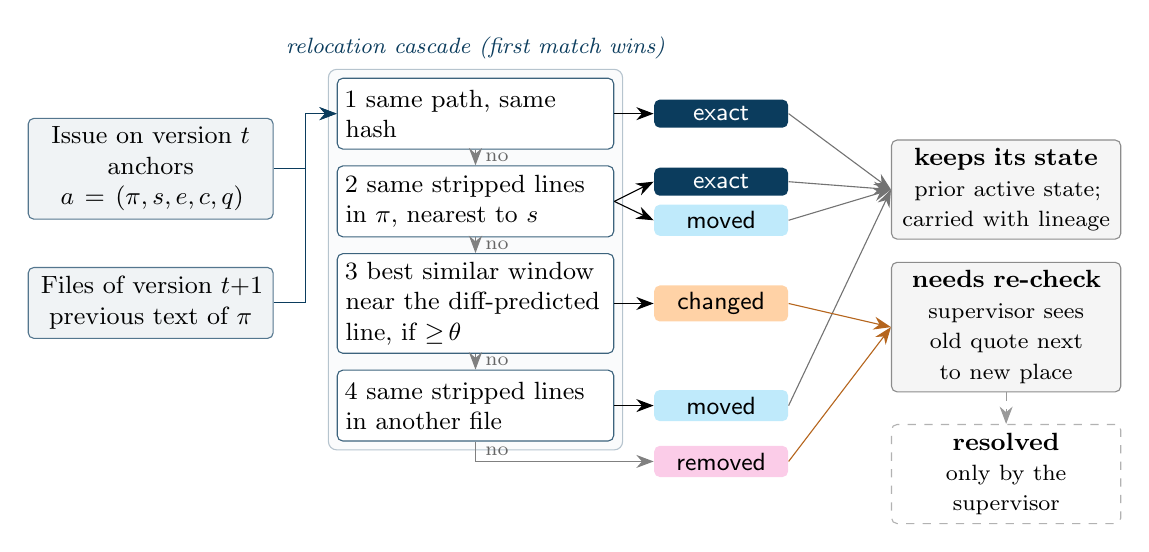
\begin{tikzpicture}[
  node distance=4mm and 5mm, >={Stealth[length=2.2mm]}, font=\small,
  box/.style={draw=ink!70, rounded corners=2pt, fill=ink!6, align=center, inner sep=3pt, minimum height=9mm},
  tier/.style={draw=ink!80, rounded corners=2pt, fill=white, align=left, inner sep=3pt, text width=33mm, minimum height=9mm},
  lbl/.style={rounded corners=2pt, align=center, inner sep=2.5pt, minimum width=17mm, font=\small\sffamily},
  st/.style={draw=black!45, rounded corners=2pt, fill=black!4, align=center, inner sep=3pt, text width=27mm}]
\node[box, text width=29mm] (old) {Issue on version $t$\\ anchors $a=(\pi,s,e,c,q)$};
\node[box, text width=29mm, below=6mm of old] (new) {Files of version $t{+}1$\\ previous text of $\pi$};
\node[tier, right=8mm of old, yshift=7mm] (t1) {1 same path, same hash};
\node[tier, below=2mm of t1] (t2) {2 same stripped lines in $\pi$, nearest to $s$};
\node[tier, below=2mm of t2] (t3) {3 best similar window near the diff-predicted line, if ${\ge}\,\theta$};
\node[tier, below=2mm of t3] (t4) {4 same stripped lines in another file};
\node[lbl, fill=ink, text=white, right=5mm of t1] (l1) {exact};
\node[lbl, fill=ink, text=white, right=5mm of t2, yshift=2.5mm] (l2a) {exact};
\node[lbl, fill=cyan!25, below=1mm of l2a] (l2b) {moved};
\node[lbl, fill=orange!35, right=5mm of t3] (l3) {changed};
\node[lbl, fill=cyan!25, right=5mm of t4] (l4) {moved};
\node[lbl, fill=magenta!20, below=3mm of l4] (l5) {removed};
\node[st, right=13mm of l2a, yshift=-1mm] (keep) {\textbf{keeps its state}\\ \footnotesize prior active state; carried with lineage};
\node[st, right=13mm of l3, yshift=-3mm] (re) {\textbf{needs re-check}\\ \footnotesize supervisor sees old quote next to new place};
\node[st, below=4mm of re, fill=white, draw=black!30, dashed] (res) {\textbf{resolved}\\ \footnotesize only by the supervisor};
\begin{scope}[on background layer]
\node[draw=ink!30, fill=ink!2, rounded corners=3pt, fit=(t1)(t4), inner sep=3pt, label={[font=\footnotesize\itshape, text=ink]above:relocation cascade (first match wins)}] {};
\end{scope}
\draw[->, ink] (old.east) -- ++(4mm,0) |- (t1.west);
\draw[->, ink] (new.east) -- ++(4mm,0) |- (t1.west);
\foreach \a/\b in {t1/t2, t2/t3, t3/t4} \draw[->, black!50] (\a.south) -- node[right, font=\scriptsize, black!60]{no} (\b.north);
\draw[->, black!50] (t4.south) |- node[pos=0.25, right, font=\scriptsize, black!60]{no} (l5.west);
\draw[->] (t1) -- (l1); \draw[->] (t2.east) -- (l2a.west); \draw[->] (t2.east) -- (l2b.west);
\draw[->] (t3) -- (l3); \draw[->] (t4) -- (l4);
\foreach \n in {l1,l2a,l2b,l4} \draw[->, black!55] (\n.east) -- (keep.west);
\foreach \n in {l3,l5} \draw[->, warn] (\n.east) -- (re.west);
\draw[->, black!40, dashed] (re.south) -- (res.north);
\end{tikzpicture}
\caption{Carry-forward of one issue. Each anchor is re-found by the first tier that matches; the issue needs a re-check if any anchor is \lbl{changed} or \lbl{removed}. No automated transition leads to \lbl{resolved}: only the supervisor closes an issue.}
\label{fig:cascade}
\end{figure*}


\subsection{Versions and Anchors}
A submission version $V_t$ contains files $(\pi,T)$ and extracted report text. A code anchor is $a=(\pi,s,e,c,q)$: path, first and last line of an original span of height $k=e-s+1$, whole-file SHA-256 digest and quoted text. Let $\qbar$ be the nonblank quoted lines with surrounding whitespace removed. The quotation is matching evidence, not a globally unique identifier of a program entity. An issue may hold up to twelve anchors. Report anchors store quoted text; media attachments can refer to an issue, a code range or the review. Their bytes are content-addressed. The original benchmark scores only code anchors and checks file/start location. Section~\ref{sec:ranges} separately evaluates AST source-line extents on surviving real-history targets.

\begin{algorithm}[t]
\caption{Relocate a code anchor $a = (\pi, s, e, c, q)$}
\label{alg:relocate}
\small
\begin{algorithmic}[1]
\Require new files $F$ (path $\mapsto$ (digest, text)); previous text $P$ of $\pi$; threshold $\theta$
\If{$\pi \in F$ \textbf{and} digest$(F[\pi]) = c$} \Return $(\pi, s, e, \lbl{exact})$
\EndIf
\State $\qbar \gets$ stripped non-blank lines of $q$; $k \gets e - s + 1$
\If{$\pi \in F$}
  \State $R \gets$ starts of runs equal to $\qbar$ in $F[\pi]$
  \If{$R \neq \emptyset$}
    \State $s' \gets \arg\min_{x \in R} |x - s|$
    \State \Return $(\pi, s', \cdot, s' = s\ ?\ \lbl{exact} : \lbl{moved})$
  \EndIf
  \State $p \gets$ image of $s$ under the line diff of $P$ and $F[\pi]$; $r \gets \max(10, 2k)$
  \State $(\rho, s') \gets \max_{x \in [p-r,\, p+r]} \mathrm{ratio}(\qbar, \mathrm{window}(F[\pi], x, k))$
  \If{$\rho \geq \theta$} \Return $(\pi, s', s' + k - 1, \lbl{changed})$
  \EndIf
\EndIf
\For{each other path $\pi'$ in $F$, in sorted order}
  \If{$\qbar$ is a run in $F[\pi']$ at $x$} \Return $(\pi', x, \cdot, \lbl{moved})$
  \EndIf
\EndFor
\State \Return \lbl{removed}
\end{algorithmic}
\end{algorithm}

\subsection{Relocation}
Given $V_{t+1}$ and, when available, the previous text of $\pi$, relocation returns a new position and a label $\ell \in \{\lbl{exact}, \lbl{moved}, \lbl{changed}, \lbl{removed}\}$ (Algorithm~\ref{alg:relocate}, Fig.~\ref{fig:cascade}). Tier~1 accepts an untouched file. Tier~2 searches $\qbar$ as a contiguous run of stripped non-blank lines in the same file and takes the occurrence nearest the old start; this tolerates re-indentation and blank-line changes and prefers the original copy when code is duplicated. Tier~3 handles edits in place. It maps the old start line through a line diff \cite{pythonsequence} of the previous and new file to an expected start $p$. It then scores every window of height $k$ starting within $p \pm r$, $r = \max(10, 2k)$, by the similarity ratio of the joined stripped lines, and accepts the best window if the ratio reaches $\theta = 0.85$. Tier~4 searches $\qbar$ in the other files, for code moved between files. Tier~3 deliberately runs before tier~4. An edited block should be recognised in place, not matched to an identical copy elsewhere. The window stays near the diff-predicted line to reduce matches to distant look-alike lines (Section~\ref{sec:results}, RQ3). A report anchor is \lbl{exact} if its normalised quotation occurs in the new report, \lbl{changed} if the most similar sentence reaches a ratio of 0.8, and \lbl{removed} otherwise.


For normalized lines joined by a single space, let $u$ and $v$ be the resulting quotation and candidate strings. The fuzzy score is
\begin{equation}
\operatorname{ratio}(u,v)=\frac{2\sum_i m_i}{|u|+|v|},
\end{equation}
where $m_i$ are the matching-block lengths returned by Python's sequence matcher with its automatic junk heuristic disabled. This is not a claim of maximum common-subsequence matching. Only valid full-height windows are considered. The implementation scans starts in ascending order and retains the first maximum; exact-run distance ties likewise select the first run. If the previous file text is unavailable, the predicted start defaults to the old start. These deterministic details affect ambiguous matches and are part of the evaluated implementation.

\subsection{State Invariant and Matching Limits}
The issue-state contract prevents relocation alone from resolving an issue; this is distinct from accurate change detection. Tier~1 reports \lbl{exact} for an unchanged file, while tier~2 can report it for an identical normalized quotation at the old start. Normalized equality does not imply semantic equivalence: in Python, re-indenting a return into a conditional can preserve its stripped text and line number while changing the syntax tree. An identical copy can also replace the original entity. A \lbl{moved} label retains the issue's active state and can therefore miss a re-check when a copy is mistaken for the target. Section~\ref{sec:definitionaudit} examines this distinction in the recorded data.

\begin{figure}[t]
\centering
% Review-issue lifecycle across versions (shared by both papers).
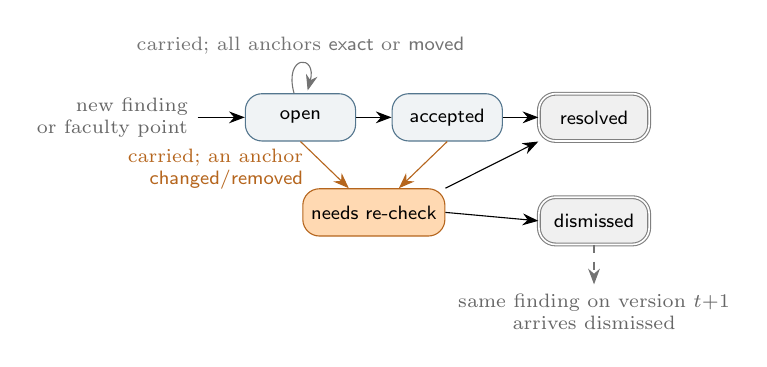
\begin{tikzpicture}[>={Stealth[length=2mm]}, font=\scriptsize, node distance=7mm and 4.5mm,
  st/.style={draw=ink!70, rounded corners=6pt, fill=ink!6, align=center, inner sep=3pt, minimum width=14mm, minimum height=6mm, font=\scriptsize\sffamily},
  fin/.style={st, fill=black!6, draw=black!50, double}]
\node[st] (open) {open};
\node[st, right=of open] (acc) {accepted};
\node[st, below=9mm of $(open)!0.5!(acc)$, fill=orange!30, draw=warn] (re) {needs re-check};
\node[fin, right=of acc] (res) {resolved};
\node[fin, below=of res] (dis) {dismissed};
\node[left=6mm of open, align=right, text=black!60] (new) {new finding\\ or faculty point};
\draw[->] (new) -- (open);
\draw[->] (open) -- (acc);
\draw[->] (acc) -- (res);
\draw[->] (re.east) -- (dis.west);
\draw[->, warn] (open.south) -- node[pos=0.6, left=6pt, text=warn, align=right]{carried; an anchor\\ \lab{changed}/\lab{removed}} (re);
\draw[->, warn] (acc.south) -- (re);
\draw[->] (re.north east) -- (res.south west);
\draw[->, black!55] (open) edge[loop above] node[above, align=center]{carried; all anchors\ \lab{exact} or \lab{moved}} (open);
\draw[->, black!55, dashed] (dis.south) -- ++(0,-5mm) node[below, align=center, text=black!60]{same finding on version $t{+}1$\\ arrives dismissed};
\end{tikzpicture}
\caption{Lifecycle of a review issue across versions. Black arrows are faculty actions, orange arrows are carry-forward. Carry-forward moves an issue to \lab{needs re-check} when any anchor is \lab{changed} or \lab{removed}, and otherwise keeps its state. Supervisors may set any state from any state; no system or assistant action resolves an issue. A new finding matching an issue dismissed on the preceding version is created dismissed, and a deleted issue is not carried (Section~\ref{sec:statecheck}).}
\label{fig:states}
\end{figure}

\subsection{Issue States}
When a new version arrives, active issues (\lbl{open}, \lbl{accepted} or \lbl{needs re-check}) are copied into its review with relocated anchors and a lineage reference. Any \lbl{changed} or \lbl{removed} anchor requests re-check; otherwise the previous active state is retained. No relocation transition resolves an issue. A finding raised again is matched to a carried issue by category, title and overlapping evidence, so that a carried concern is not duplicated. A newly raised finding is also compared with the findings dismissed on the immediately preceding version, by category and the first paragraph of its description (first 200 normalised characters); a match is created already dismissed, with a note naming that version. The key is a heuristic: findings that share an opening paragraph are conflated, rewording evades it, and the memory lapses if a version does not raise the finding (Section~\ref{sec:statecheck}). Fig.~\ref{fig:states} summarizes the lifecycle.

\subsection{Media Notes and Release}
Notes attached to carried issues follow their issue; notes pinned to code are re-found by the cascade. A note whose code is gone is kept on the review as a whole and records where it was (``it was on \emph{path:lines}''). At publication, notes on issues the supervisor shares are listed in each student's immutable feedback snapshot, and the file route serves a note only to students whose snapshot lists it.

% System architecture section (shared by paper.tex and paper-ieee.tex).
\section{System Architecture}\label{sec:impl}

\sys{} is the resubmission model of the review page of a capstone review portal used by faculty supervisors and student teams. It is not a separate service: the cascade, the issue states and the media-note rules run inside the portal's review composition, against the same database and file store as the rest of the review. This section describes the implemented architecture (Fig.~\ref{fig:deploy}), the data the method reads and writes (Fig.~\ref{fig:model}), how a review is composed for a new version (Algorithm~\ref{alg:compose}), and the integrity properties that the evaluation does not measure but the design depends on.

\begin{figure*}[t]
\centering
% Deployment architecture of the review portal with the Living Review components highlighted (shared by both papers).
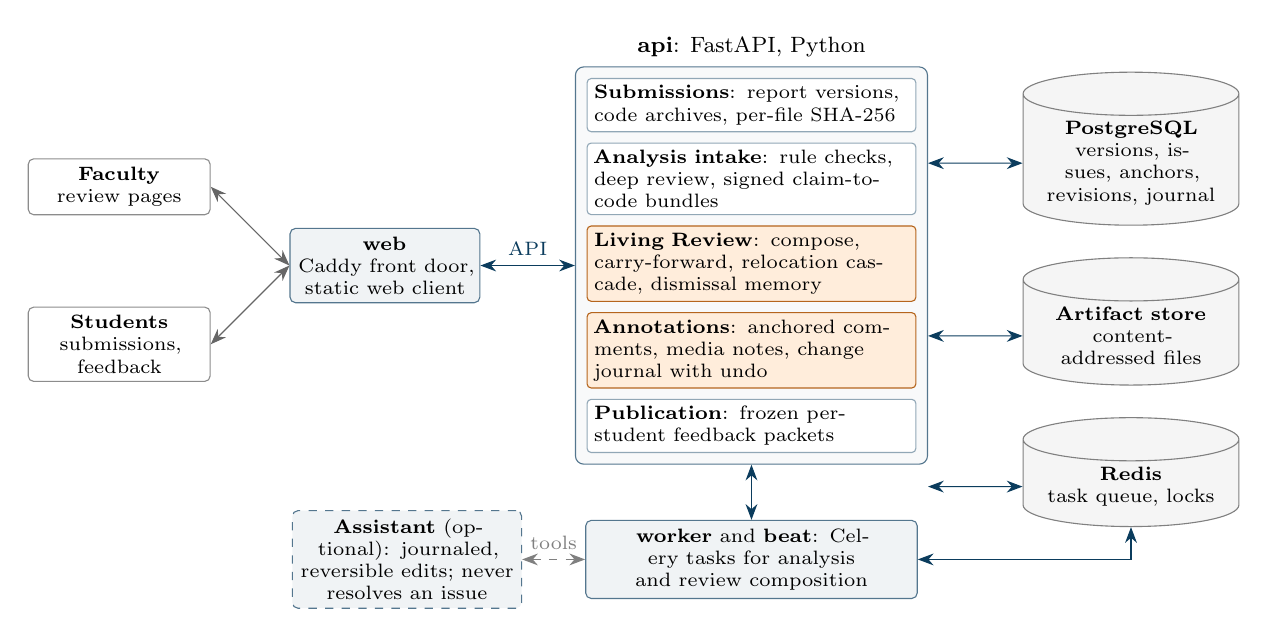
\begin{tikzpicture}[>={Stealth[length=2mm]}, font=\footnotesize,
  user/.style={draw=black!45, rounded corners=2pt, fill=white, align=center, inner sep=3pt, text width=21mm, font=\scriptsize},
  comp/.style={draw=ink!70, rounded corners=2pt, fill=ink!6, align=center, inner sep=3pt, font=\scriptsize},
  mod/.style={draw=ink!45, rounded corners=1.5pt, fill=white, align=left, inner sep=2.5pt, text width=40mm, font=\scriptsize},
  lr/.style={mod, fill=orange!14, draw=warn},
  store/.style={draw=black!50, cylinder, shape border rotate=90, aspect=0.2, fill=black!4, align=center, inner sep=2pt, text width=26mm, font=\scriptsize}]
\node[mod] (m1) at (0,0) {\textbf{Submissions}: report versions, code archives, per-file SHA-256};
\node[mod, below=1.3mm of m1] (m2) {\textbf{Analysis intake}: rule checks, deep review, signed claim-to-code bundles};
\node[lr, below=1.3mm of m2] (m3) {\textbf{Living Review}: compose, carry-forward, relocation cascade, dismissal memory};
\node[lr, below=1.3mm of m3] (m4) {\textbf{Annotations}: anchored comments, media notes, change journal with undo};
\node[mod, below=1.3mm of m4] (m5) {\textbf{Publication}: frozen per-student feedback packets};
\begin{scope}[on background layer]
\node[draw=ink!70, rounded corners=3pt, fill=ink!3, fit=(m1)(m5), inner sep=4pt, label={[font=\footnotesize]above:\textbf{api}: FastAPI, Python}] (api) {};
\end{scope}
\node[comp, text width=22mm, left=12mm of api] (web) {\textbf{web}\\Caddy front door,\\static web client};
\node[user, left=10mm of web, yshift=10mm] (fac) {\textbf{Faculty}\\review pages};
\node[user, left=10mm of web, yshift=-10mm] (stu) {\textbf{Students}\\submissions, feedback};
\node[store, right=12mm of api, yshift=13mm] (pg) {\textbf{PostgreSQL}\\versions, issues, anchors,\\revisions, journal};
\node[store, below=4mm of pg] (art) {\textbf{Artifact store}\\content-addressed files};
\node[store, below=4mm of art] (redis) {\textbf{Redis}\\task queue, locks};
\node[comp, text width=40mm, below=7mm of api] (worker) {\textbf{worker} and \textbf{beat}: Celery tasks for analysis and review composition};
\node[comp, dashed, text width=27mm, left=8mm of worker] (asst) {\textbf{Assistant} (optional): journaled, reversible edits; never resolves an issue};
\draw[<->, black!60] (fac.east) -- (web.west);
\draw[<->, black!60] (stu.east) -- (web.west);
\draw[<->, ink] (web) -- node[above, font=\scriptsize]{API} (api);
\draw[<->, ink] (api.east |- pg) -- (pg.west);
\draw[<->, ink] (api.east |- art) -- (art.west);
\draw[<->, ink] (api.east |- redis) -- (redis.west);
\draw[<->, ink] (worker.east) -| (redis.south);
\draw[<->, ink] (worker) -- (api);
\draw[<->, black!50, dashed] (asst) -- node[above, font=\scriptsize]{tools} (worker.west);
\end{tikzpicture}
\caption{Architecture of the review portal. Faculty and students reach the portal through one front door. Caddy serves the static client and the api container provides protected application routes; components that implement \sys{} are shaded orange. Durable state lives in PostgreSQL and a content-addressed artifact store; analysis and review composition also run as queued worker tasks. The optional assistant can edit a draft only through journaled, reversible tool calls.}
\label{fig:deploy}
\end{figure*}

\subsection{Deployment}
The portal runs as a small set of containers. A web container is the single front door: Caddy serves the static web client used by faculty and students and proxies API calls. The api container runs the FastAPI application, which owns authentication, authorisation on every protected route, validation and all durable state. A worker and a scheduler run Celery tasks on a Redis queue: analysis of a submission (rule checks, a deep review and the partner claim-to-code tracer, whose results arrive as signed bundles) and the composition of the review. PostgreSQL holds versions, review issues, anchors, revisions, the change journal and publications; schema changes are forward-only migrations. Submitted archives, extracted files and media notes are kept in an artifact store addressed by their SHA-256 digest. An optional assistant runs as its own service and can create, edit and delete review points through journaled, undoable tool calls, but cannot publish, and a resolve or dismiss it suggests takes effect only when a supervisor applies it. Relocation needs no extra component: its matching core uses Python's standard-library sequence matcher \cite{pythonsequence}.

\begin{figure*}[t]
\centering
% Data model behind the Living Review (shared by both papers); names follow the portal's tables.
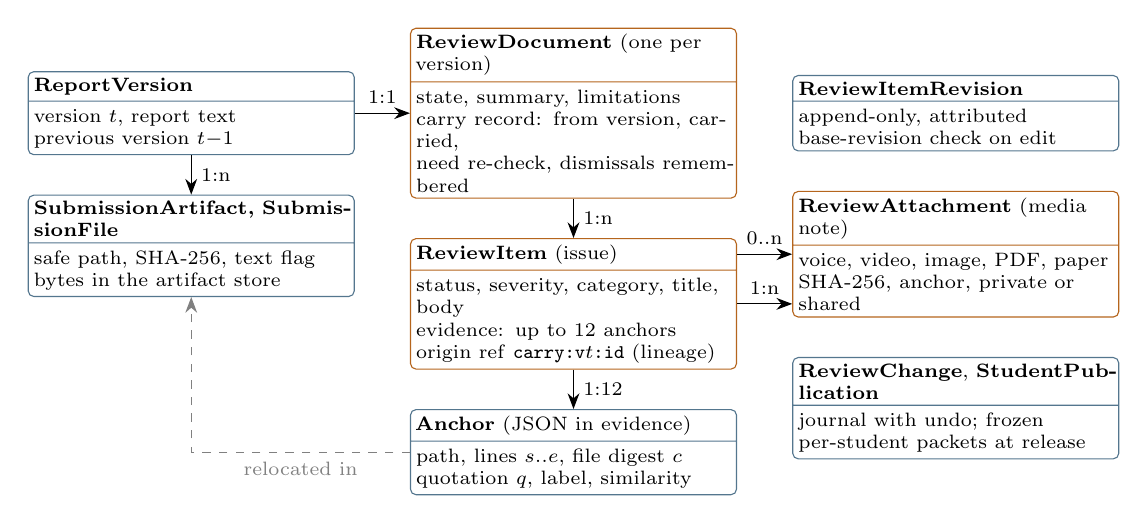
\begin{tikzpicture}[>={Stealth[length=2mm]}, font=\scriptsize, node distance=5mm and 7mm,
  ent/.style={draw=ink!70, rounded corners=2pt, fill=white, align=left, inner sep=2pt, text width=40mm,
    rectangle split, rectangle split parts=2, rectangle split part fill={ink!12,white}},
  lr/.style={ent, draw=warn, rectangle split part fill={orange!22,white}}]
\node[ent] (ver) {\textbf{ReportVersion}\nodepart{two}\strut version $t$, report text\\ previous version $t{-}1$};
\node[ent, below=of ver] (art) {\textbf{SubmissionArtifact, SubmissionFile}\nodepart{two}\strut safe path, SHA-256, text flag\\ bytes in the artifact store};
\node[lr, right=of ver] (doc) {\textbf{ReviewDocument} (one per version)\nodepart{two}\strut state, summary, limitations\\ carry record: from version, carried,\\ need re-check, dismissals remembered};
\node[lr, below=of doc] (item) {\textbf{ReviewItem} (issue)\nodepart{two}\strut status, severity, category, title, body\\ evidence: up to 12 anchors\\ origin ref \texttt{carry:v$t$:id} (lineage)};
\node[ent, right=of doc] (rev) {\textbf{ReviewItemRevision}\nodepart{two}\strut append-only, attributed\\ base-revision check on edit};
\node[lr, below=of rev] (att) {\textbf{ReviewAttachment} (media note)\nodepart{two}\strut voice, video, image, PDF, paper\\ SHA-256, anchor, private or shared};
\node[ent, below=of item] (anc) {\textbf{Anchor} (JSON in evidence)\nodepart{two}\strut path, lines $s..e$, file digest $c$\\ quotation $q$, label, similarity};
\node[ent, below=of att] (pub) {\textbf{ReviewChange}, \textbf{StudentPublication}\nodepart{two}\strut journal with undo; frozen\\ per-student packets at release};
\draw[->] (ver) -- node[above]{1:1} (doc);
\draw[->] (ver) -- node[right]{1:n} (art);
\draw[->] (doc) -- node[right]{1:n} (item);
\draw[->] (item) -- node[above]{1:n} (rev.west |- item.east);
\draw[->] (item) -- node[right]{1:12} (anc);
\draw[->] (item.east |- att.west) -- node[above]{0..n} (att.west);
\draw[->, dashed, black!50] (anc.west) -| node[pos=0.25, below]{relocated in} (art.south);
\end{tikzpicture}
\caption{Data model behind \sys{} (simplified; names follow the portal's tables). Orange entities are written by carry-forward. A carried issue is a new row in the next version's review whose origin reference names the version and issue it came from; its anchors are re-found in that version's files.}
\label{fig:model}
\end{figure*}

\subsection{Data Model}
A report version records its predecessor, so the versions of a project form a chain (Fig.~\ref{fig:model}). The files of a version are rows with a safe path, a SHA-256 digest and a text flag; their bytes stay in the artifact store, and only text files below a size limit are read for relocation. Each version has one review document, which holds the supervisor's review: issues, a summary, stated limitations and a carry record (from which version issues were carried, how many need a re-check, how many dismissals were remembered). An issue has a status among \lab{open}, \lab{accepted}, \lab{needs re-check}, \lab{resolved} and \lab{dismissed}, a severity, a category, a title and body, and up to twelve anchors stored as JSON in its evidence. A carried issue's origin reference has the form \texttt{carry:v$t$:id}; it records the issue's lineage and makes composition idempotent. Every edit of an issue appends an attributed revision, and a write must name the revision it was based on, so concurrent edits are detected rather than lost. Media notes are attachment rows that point to bytes stored once under their digest; a note is anchored to an issue, to a code range or to the whole review, and is private or shared. A per-version change journal records every write by faculty, the system or the assistant, and supports undo. At release, the approved shared points are frozen into a packet per student.

\begin{algorithm}[t]
\caption{Compose the review of version $t{+}1$}
\label{alg:compose}
\small
\begin{algorithmic}[1]
\Require version $t{+}1$ with files $F$ and report text; review $D_t$ of version $t$; new findings $\Phi$
\State lock version $t{+}1$; $D \gets$ its review document (created if absent)
\State $K \gets$ keys (category, first description paragraph) of issues \lab{dismissed} in $D_t$
\For{each issue $i \in D_t$ that is \lab{open}, \lab{accepted} or \lab{needs re-check}}
  \If{$D$ already holds an issue with origin \texttt{carry:v$t$:}$i$} \textbf{continue} \EndIf
  \State $A \gets$ anchors of $i$ re-found in $F$ (Algorithm~\ref{alg:relocate}) or in the report text
  \State $s \gets$ \lab{needs re-check} \textbf{if} any anchor in $A$ is \lab{changed} or \lab{removed} \textbf{else} status of $i$
  \State add a copy of $i$ to $D$ with anchors $A$, status $s$ and origin \texttt{carry:v$t$:}$i$
\EndFor
\For{each finding $f \in \Phi$}
  \If{a carried issue has $f$'s category and title and an overlapping anchor}
    \State refresh its anchors; if it is active, set it to \lab{needs re-check}
  \ElsIf{the key of $f$ is in $K$} \State add $f$ as \lab{dismissed}, naming the version where it was dismissed
  \Else \State add $f$ as \lab{open}
  \EndIf
\EndFor
\State carry media notes: with their carried issue, or re-found by Algorithm~\ref{alg:relocate}
\State record the carry counts for the banner; mark $D$ ready
\end{algorithmic}
\end{algorithm}

\subsection{Review Composition}
When a version arrives, the worker analyses it and the review is composed (Algorithm~\ref{alg:compose}). Composition first locks the version's row, because the faculty home page, open project tabs and the worker may all compose the same version at once. Carry-forward comes first, so that a finding the new analysis raises again is matched to the issue the supervisor already has rather than duplicated. Carry-forward reads only the immediately preceding version's review; if that review was never composed, its issues reach the next version only after it is composed and the later version recomposed. If the new finding has the same category and title as a carried issue and an overlapping anchor, the carried issue keeps the supervisor's wording and takes the fresh evidence; an active issue asks for a re-check, and a resolved or dismissed one keeps its state. If it matches an issue the supervisor dismissed on the previous version, it is created already dismissed, with a note naming that version. Media notes follow: a note attached to a carried issue moves with it; a note pinned to code is re-found by the cascade and, when its code is gone, stays on the whole review with a note of where it was. A copy is a new row that points to the same stored bytes. Finally the carry counts are recorded, and the review page shows them as a banner (``$N$ points carried over $\cdot$ $M$ need a re-check''), with a ``From version~$n$'' tag on each carried issue and a plain-language note on each anchor.

\subsection{Integrity Properties}
Five properties govern workflow integrity.
\emph{Idempotence:} composition never overwrites an existing issue and recognises carried issues by their origin reference, so running it again, for example after a late partner analysis, yields the same review and keeps every faculty edit.
\emph{Attribution and undo:} every change to an issue, summary, note or attachment is an attributed, append-only revision and journal entry; undo appends a restoring entry and is refused when a newer change touched the same target.
\emph{Verified quotations:} a selection made in the review page becomes an anchor only after its quotation has been verified against text the server read from the stored version, so an anchor never quotes text that was not submitted.
\emph{Separation of private and shared feedback:} private notes never enter a student packet; at release the approved shared wording is frozen, and a student can open source only through an anchor in their own packet whose file digest still matches.
\emph{Bounded automation:} neither composition nor the assistant can mark an issue resolved; settling an issue is always an explicit faculty action (Fig.~\ref{fig:states}).

\subsection{Implementation and Tests}
The portal implementation uses Python, FastAPI, SQLAlchemy and PostgreSQL. Its test sources exercise submission, faculty dismissal, anchored notes, revision requests and subsequent carry-forward; they also cover attachment scoping and publication. These are integration checks with a different purpose from the relocation benchmarks. This paper does not report an independent live-deployment audit or a measured faculty session. The evaluated relocation functions come from the pinned source snapshot used by the benchmark; later application changes must not be assumed to share its results.

\section{Evaluation Method}
\label{sec:method}

\subsection{Corpus}
We used every Python file of 60--1,500 lines in the backend of the review portal and in a partner team's claim-to-code tracer, exported from fixed commits so that the corpus does not drift with development: \nFiles{} files and \nLines{} lines. The code is real, maintained application code, not generated text.

\begin{table}[t]
\caption{Edit Types and Ground Truth}
\label{tab:edits}
\centering
\footnotesize
\setlength{\tabcolsep}{4pt}
\begin{tabular}{@{}lll@{}}
\toprule
Edit & What happens & Correct outcome \\
\midrule
no change & file untouched & same lines \\
edit elsewhere & one distant line edited & same lines \\
insert / delete above & 1--40 / 1--15 lines & shifted lines \\
re-indent & anchor indented 4 spaces & same lines \\
move in file & block moved $>$30 lines & new location \\
move to other file & block moved to file $\pi'$ & new file, location \\
duplicate above & copy inserted $\geq$40 above & shifted original \\
\midrule
token edit & one identifier renamed & same lines \\
insert + token edit & both & shifted lines \\
rewrite & replaced by other code & reported gone \\
delete & block deleted & reported gone \\
\bottomrule
\multicolumn{3}{@{}p{0.95\columnwidth}@{}}{\scriptsize The first eight preserve the anchored content; the last four change it.}
\end{tabular}
\end{table}


\subsection{Trials and Ground Truth}
A trial picks a file and a 1--10-line anchor. It starts on a nonblank line, contains at least 30 non-space characters, has distinct lines and has a quotation unique in the source file. One of twelve edit operators supplies a reference start location or a gone target (Table~\ref{tab:edits}). Inserted filler is copied from other corpus files. Up to twenty-five additional sampled files accompany the edited version. There are \nPerOp{} trials per operator and \nTrials{} per seed. The main and replication seeds are \seedMain{} and \seedRep. A separate tuning seed, 7, supplies 150 trials per operator. The default threshold was fixed for the reported main runs; no externally registered protocol is documented here. These are controlled text mutations of real source, not necessarily valid or behavior-preserving Python programs.

\subsection{Baselines}
The comparators are implemented policies, not executions of commercial review products. \emph{Fixed line} retains the original path and span and returns no match if the normalized quotation differs there. \emph{Diff drift} follows equal line-diff blocks but returns no match if an anchored line changes or the range ceases to be contiguous. \emph{Exact quote} searches the same file for the nearest stripped quotation. These three policies do not attempt fuzzy recovery of edited quotations. \emph{Cascade v1}, an earlier internal version, is a stronger comparator than these three policies: it searches other paths before fuzzy matching, searches the whole original file and uses $\theta=0.75$. It differs from the final default in three respects, so its default comparison is compound rather than a single-factor ablation. Equal-threshold comparisons separate out threshold choice but still change order and scope together. The original LHDiff binary and GumTree are not benchmarked. A separately pinned third-party hybrid tracker is evaluated on controlled trials in Section~\ref{sec:externaltracker} and retained real-history observations in Section~\ref{sec:realtracker}.

\subsection{Outcomes and Metrics}
A location is correct if its file and starting line equal the reference, or if it returns no match when the reference target is gone. It is lost if the target survives but no location is accepted, and wrong if it is placed elsewhere. The original scoring function does not check the returned end line, range overlap or continued relevance of the review concern; the added range analysis in Section~\ref{sec:ranges} addresses the first two on a defined subset. The benchmark's \emph{silent error} means a returned location labelled unchanged under its fixed-height normalized-quote definition when the quote changed or the location is wrong; for the cascade this corresponds to an erroneous \lbl{exact} label. A \lbl{moved} label can still fail to trigger re-check. We therefore report the exact-label count alongside re-check recall and a second reference definition. Synthetic proportions use nominal 95\% Wilson score intervals \cite{wilson1927probable}.

For paired correctness, $b_{01}$ counts trials correct only for the final cascade and $b_{10}$ counts trials correct only for the comparator. McNemar's framework compares the discordant pairs \cite{mcnemar1947note}. Conditional on $d=b_{01}+b_{10}$, the null assigns each direction probability $1/2$. The archived implementation computes the two-sided exact binomial tail
\begin{equation}\label{eq:pairedexact}
p=\min\left\{1,\;2\sum_{j=0}^{\min(b_{01},b_{10})}\binom{d}{j}2^{-d}\right\},
\end{equation}
with $p=1$ when $d=0$. This specifies the calculation reported in Table~\ref{tab:overall}. These nominal trial-level calculations do not model source-file or project dependence. Runtime is measured per relocation on one laptop core, not per complete review.


\section{Controlled Edit Results}
\label{sec:results}


\subsection{RQ1: Start-Location Accuracy}
\begin{table*}[t]
\caption{Overall Results on \nTrials{} Trials (Seed \seedMain)}
\label{tab:overall}
\centering
\small
\tablenote{\begin{tabular}{@{}lcccccc@{}}\toprule
Method & Correct \% [95\% CI] & Wrong & Lost & Paired vs.\ ours & Replication & ms (median / p95) \\
 & seed \seedMain & lines \% & \% & $b_{01}/b_{10}$, $p$ & seed \seedRep & \\ \midrule
Cascade (ours) & 98.5 [98.0, 98.8] & 1.5 & 0.1 & --- & 98.6 & 0.08 / 65.1 \\
Cascade v1 (internal) & 96.4 [95.7, 96.9] & 3.6 & 0.0 & 84/8, $<10^{-16}$ & 97.1 & 0.07 / 498.4 \\
\midrule
Exact quote & 74.9 [73.4, 76.3] & 0.3 & 24.9 & 868/18, $<10^{-16}$ & 74.9 & 0.05 / 0.2 \\
Diff drift & 58.3 [56.7, 59.9] & 0.0 & 41.7 & 1465/20, $<10^{-16}$ & 58.3 & 0.26 / 1.8 \\
Fixed line & 41.7 [40.1, 43.3] & 0.0 & 58.3 & 2065/20, $<10^{-16}$ & 41.7 & 0.02 / 0.1 \\
\bottomrule
\end{tabular}}{The paired column gives the trials only the cascade got right ($b_{01}$) and only the other method got right ($b_{10}$), with the two-sided exact McNemar $p$. The replication column repeats the whole benchmark with seed \seedRep.}
\end{table*}

\begin{figure*}[t]
\centering
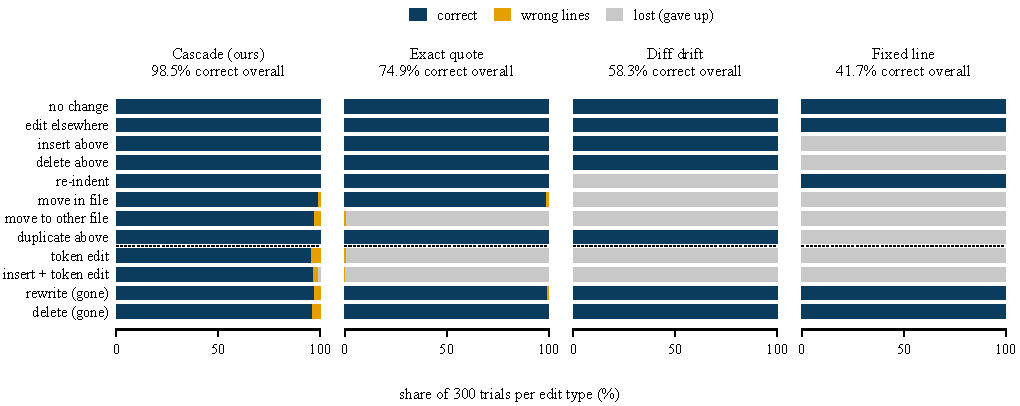
\includegraphics[width=\textwidth]{figures/per-op-v3.pdf}
\caption{Outcome per edit type for each method (\nPerOp{} trials per bar, seed \seedMain; dashed line separates edits that preserve the anchored content from edits that change it). Baselines fail by giving up (grey): the fixed-line policy loses every shifted anchor, diff drift every anchor whose lines were touched (including a pure re-indent), exact quotes every edited anchor and every anchor moved to another file. The cascade's failures are mostly wrong placements (orange); an erroneous moved label can still miss workflow re-check (Section~\ref{sec:results}, RQ2).}
\label{fig:outcomes}
\end{figure*}
The cascade reached a correct outcome on \casCorrect\% of trials (95\% CI \casLo--\casHi; Table~\ref{tab:overall}); its placement on surviving anchors, the Place column of Table~\ref{tab:safety}, was \smCtlCasPlacePct\%. Exact-quote search reached \qeCorrect\%, diff drift \ddCorrect\% and the fixed-line policy \lnCorrect\%. The reported paired tests detect differences on these trials: exact quotes were right on only \qeOnlyOther{} trials where the cascade was not, against \qeOnlyCas{} the other way. Fig.~\ref{fig:outcomes} and Table~\ref{tab:pertype} show where the gap comes from. The baselines seldom place an anchor on wrong lines; they fail by giving up. These losses describe the implemented policies and do not estimate the behavior of a complete review product.

The fixed-line and diff-drift policies succeed on exactly five and seven controlled edit types, respectively, explaining their unchanged scores across seeds. Exact-quote outcomes can also depend on quotation ambiguity. The cascade's \casWrong\% wrong placements fall in three groups. For code moved to another file (\casWrongMoveFile\%), a similar window near the old place is taken as an in-place edit. For token edits (\casWrongEditToken\%) and insert-plus-edit (\casWrongInsertAndEdit\%), an adjacent look-alike window scores higher than the edited original. For code that was rewritten or deleted (\casWrongRewrite\% and \casWrongDeleteBlock\%), a similar window near the old place passes the threshold, or an identical copy exists in another file. The three original quotation-based methods are misled in the same \casWrongMoveWithin\% of in-file moves. This is consistent with a copy of the block that differs only in whitespace lying closer to the old position, a residual ambiguity of the benchmark rather than of any one method.

\subsection{RQ2: Labels and Re-checks}
\begin{figure}[t]
\centering
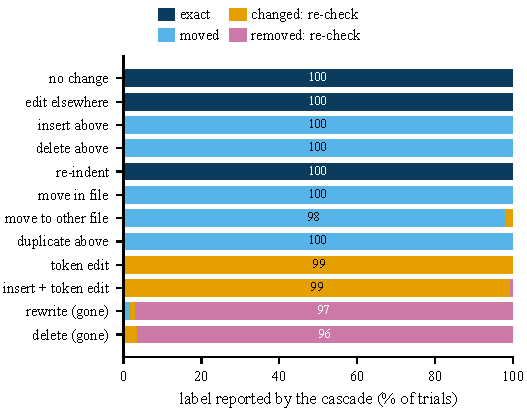
\includegraphics[width=\columnwidth]{figures/labels-v3.pdf}
\caption{Label reported by the cascade per edit type (seed \seedMain). Orange and pink labels send the issue back to the supervisor; blue labels keep its state.}
\label{fig:labels}
\end{figure}
Across \nTrialsAll{} generated observations, no method produced a silent error under the original quote-window score. The nominal Wilson upper bound of \silentUB\% assumes independent Bernoulli trials and is not a semantic-error bound or a project-level guarantee. On the main seed, \nMissedRecheck{} of \nContentChanged{} changed observations were labelled \lbl{moved} to an identical copy elsewhere and did not request re-check (\missedRecheck\%). Among \nUnchanged{} preserved observations, \nFalseRecheck{} requested re-check (\falseRecheck\%), all cross-file moves matched to nearby edits. Re-check precision was \recheckPrecision\%. These label outcomes are separate from location correctness and from human recognition of the underlying concern (Fig.~\ref{fig:labels}).

\subsection{RQ3: Combined Design}
\begin{figure*}[t]
\centering
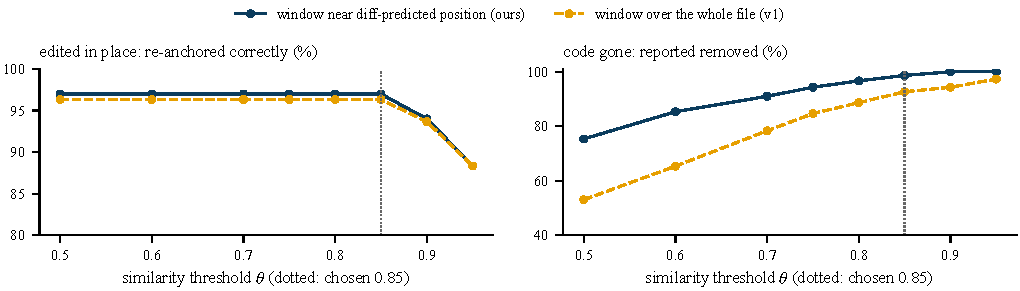
\includegraphics[width=\textwidth]{figures/threshold-v3.pdf}
\caption{Fuzzy-tier threshold on the separate tuning seed (seed 7, 150 trials per edit type). Left: anchors edited in place that are re-anchored correctly. Right: anchors whose code is gone that are correctly reported \lbl{removed} rather than attached to look-alike lines. Dotted line: the reported default $\theta = 0.85$; no dated prospective protocol is available.}
\label{fig:threshold}
\end{figure*}
The compound comparator changes search scope, tier order and threshold together (Table~\ref{tab:overall}, \emph{Cascade v1}). Cascade v1 recovers slightly more cross-file moves (\voneMoveFile\% against \casMoveFile\%) under its combined settings. However, it placed rewritten and deleted anchors on look-alike code elsewhere in the file: \voneWrongRewrite\% and \voneWrongDeleteBlock\% of them, against \casWrongRewrite\% and \casWrongDeleteBlock\% for the final order. Overall the final design is better by \casCorrect\% to \voneCorrect\% ($b_{01}/b_{10} = \voneOnlyCas/\voneOnlyOther$, $p$\,\voneP). Fig.~\ref{fig:threshold} shows the threshold study on the tuning seed. The whole-file variant attaches more removed anchors to look-alike code at thresholds that recover genuine edits. In the final design, $\theta = 0.85$ keeps both tuning curves high; above about 0.9, genuine edits increasingly return no match. These comparisons do not separate window scope from tier order.

\subsection{RQ4: Robustness and Cost}
\begin{figure*}[t]
\centering
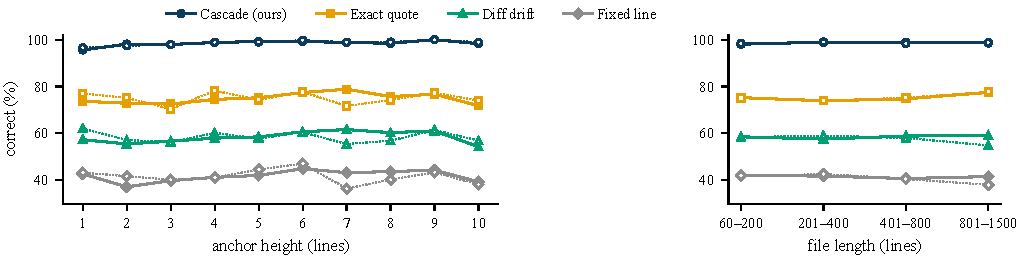
\includegraphics[width=\textwidth]{figures/robustness-v3.pdf}
\caption{Correct outcome by anchor height (left) and file length (right). Solid lines and filled markers: main seed; dotted lines and open markers: replication seed.}
\label{fig:robust}
\end{figure*}
On the fresh replication seed the cascade reached \casRep\%, against \qeRep\%, \ddRep\% and \lnRep\% for the baselines (Table~\ref{tab:overall}). Accuracy stayed between \casSpanMin\% and \casSpanMax\% across anchor heights of 1--10 lines and between \casSizeMin\% and \casSizeMax\% across file-length bands (Fig.~\ref{fig:robust}). One-line anchors are the hardest case (\casSpanOne\%), because a single edited line has many look-alikes nearby. The median relocation took \casMed\,ms (95th percentile \casPninetyfive\,ms, maximum \casMax\,ms). Tier~3 is the only expensive step, and it scores at most $2r+1$ windows. These per-anchor times do not establish whole-review or end-to-end latency; hardware, runtime configuration and review size must be specified before making that comparison.


\subsection{RQ1: Independent Hybrid Tracker}\label{sec:externaltracker}
The three policy baselines do not attempt general recovery of edited lines. To test whether the aggregate advantage persists against an independently implemented contextual tracker, we added an exploratory comparison with the MIT-licensed Go implementation by Oselvar \cite{oselvarlhdiff}. This implementation cites LHDiff and combines line-content Levenshtein similarity with surrounding-context cosine similarity. It is not the original paper authors' binary: its documentation states that it omits SimHash optimization and line-splitting support. We pinned revision \texttt{5a9f7fd} and used its command-line defaults: four context lines, content/context weights of 0.6/0.4 and the implementation's 0.45 combined-similarity cutoff. No threshold was tuned on our trials.

The adapter asks for a mapping of the old anchor's first line in the same path. A missing first-line mapping returns no match. This follows the original benchmark's path-and-start scoring; neither method receives credit for end-range validity. The tracker has no cross-file search or review-state policy. We therefore compare location outcomes only, and report cross-file and within-file strata separately. The original corpus, operators and seeds are unchanged. Trial metadata and the cascade outcomes are checked against the independently reproduced runs, and all 7,200 tracker outcomes are retained. Upstream tests and the adapter's one-based coordinate check pass. Go and Python timings are not compared, since the adapter adds inter-process communication and the implementations use different runtimes.

\begin{table}[t]
\caption{Independent Tracker on the Controlled Benchmark}\label{tab:externaltracker}
\centering\footnotesize
\begin{tabular}{@{}llrr@{}}\toprule
Stratum & Method & Main & Replication \\
 & & correct \% & correct \% \\
\midrule
All ($n=3,600$) & Cascade & 98.5 & 98.6 \\
 & Hybrid tracker & 91.3 & 91.5 \\
Within-file ($n=3,300$) & Cascade & 98.6 & 98.8 \\
 & Hybrid tracker & 99.6 & 99.8 \\
Cross-file ($n=300$) & Cascade & 97.0 & 96.3 \\
 & Hybrid tracker & 0.0 & 0.0 \\
\bottomrule
\end{tabular}
\par\smallskip
\parbox{\columnwidth}{\scriptsize Denominators are per seed. The independent tracker is a pinned third-party implementation with same-file scope. All outcomes use the benchmark's existing start-location criterion. Its lack of cross-file recovery is reported explicitly rather than interpreted as poor within-file matching.}
\end{table}

The tracker correctly handles 3,288 of 3,600 main observations, 91.3\% (nominal Wilson interval 90.4--92.2), versus 3,545 for the cascade. The paired counts are 299 correct only for the cascade and 42 correct only for the tracker. On the replication seed, the tracker handles 3,293 observations (91.5\%, interval 90.5--92.3). However, it loses all 300 cross-file targets in each seed because they are outside its scope. Among the other 3,300 observations, it correctly handles 3,288 (99.6\%) versus 3,254 (98.6\%) for the cascade on the main seed, and 3,293 versus 3,260 on replication. In-place token edits also favor the independent implementation: it recovers 588 of 600 token-edit and insertion-plus-edit targets on the main seed, versus 577 for the cascade.

The overall difference therefore reflects task scope and the benchmark's equal operator weights, not universal superiority of the cascade's within-file matching. The independent tracker is stronger on the within-file subset. Its implementation limits mean that neither this comparison nor the real-history extension in Section~\ref{sec:realtracker} establishes the performance of the canonical LHDiff algorithm. The integration can in principle use a stronger within-file tracker while retaining lineage and human resolution, but that substitution has not been evaluated here.

\section{Real-History Evaluation}
\label{sec:real}

The synthetic benchmark controls every edit, but its twelve operators and their uniform mix are our choice. To test the findings on edits nobody designed (RQ5), we repeated the comparison on the version histories of nine Python projects, \rCommits{} first-parent commits in total. Four come from our group: the review portal itself, a partner team's claim-to-code tracer, a language-model training system and an evidence-ingestion system (\rOwnCommits{} commits, a small group of developers). Five are widely used open-source libraries: Requests, Flask, Click, HTTPX and Rich. We made shallow clones of each default branch (depth 400), which gave \rOssCommits{} first-parent commits written by about a thousand contributors (\rOssAuthors{} names, counted per project). The source was only parsed, never executed. Fig.~\ref{fig:realpipe} summarises the procedure. Pairwise accuracy and re-checks address RQ5 and RQ2; definition sensitivity and complete-source checks explain their reference limits (Sections~\ref{sec:definitionaudit} and~\ref{sec:sourcecontext}). Calibration examines RQ3, followed by independent tracking, full-range recovery and ten-hop replay (Sections~\ref{sec:realtracker}--\ref{sec:chains}).


\begin{figure}[t]
\centering
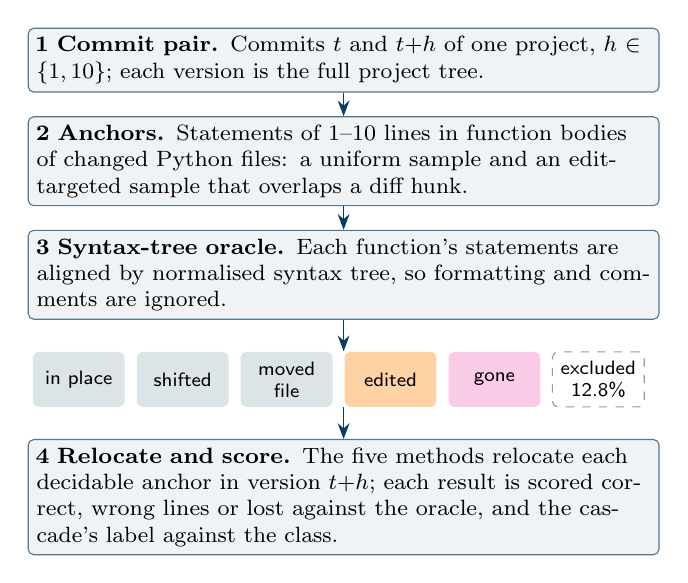
\begin{tikzpicture}[>={Stealth[length=2mm]}, font=\footnotesize, node distance=3mm,
  stage/.style={draw=ink!70, rounded corners=2pt, fill=ink!6, align=left, inner sep=3pt, text width=78mm},
  cls/.style={rounded corners=2pt, align=center, inner sep=1.5pt, minimum height=7mm, text width=10.6mm, font=\scriptsize\sffamily}]
\node[stage] (pair) {\textbf{1 Commit pair.} Commits $t$ and $t{+}h$ of one project, $h\in\{1,10\}$; each version is the full project tree.};
\node[stage, below=of pair] (anc) {\textbf{2 Anchors.} Statements of 1--10 lines in function bodies of changed Python files: a uniform sample and an edit-targeted sample that overlaps a diff hunk.};
\node[stage, below=of anc] (orc) {\textbf{3 Syntax-tree oracle.} Each function's statements are aligned by normalised syntax tree, so formatting and comments are ignored.};
\node[cls, fill=ink!14, below=4mm of orc.south west, anchor=north west, xshift=0.6mm] (c1) {in place};
\node[cls, fill=ink!14, right=1.4mm of c1] (c2) {shifted};
\node[cls, fill=ink!14, right=1.4mm of c2] (c3) {moved file};
\node[cls, fill=orange!35, right=1.4mm of c3] (c4) {edited};
\node[cls, fill=magenta!20, right=1.4mm of c4] (c5) {gone};
\node[cls, draw=black!40, dashed, right=1.4mm of c5] (c6) {excluded \rExcludedPct\%};
\node[stage, below=4mm of c1.south west, anchor=north west, xshift=-0.6mm] (run) {\textbf{4 Relocate and score.} The five methods relocate each decidable anchor in version $t{+}h$; each result is scored correct, wrong lines or lost against the oracle, and the cascade's label against the class.};
\draw[->, ink] (pair) -- (anc);
\draw[->, ink] (anc) -- (orc);
\draw[->, ink] (orc.south) -- (orc.south |- c3.north);
\draw[->, ink] (orc.south |- c3.south) -- (run.north -| orc.south);
\end{tikzpicture}
\caption{Real-history procedure. Reference locations come from syntax-tree alignment; anchors the oracle cannot decide are excluded for every method.}
\label{fig:realpipe}
\end{figure}


\subsection{Commit Pairs and Anchors}
We formed pairs of consecutive commits (a small revision) and non-overlapping pairs ten commits apart (a second, larger revision horizon). In each pair, anchors are statements of 1--10 lines directly inside function bodies of Python files the later commit modified, renamed or deleted, under the constraints of Section~\ref{sec:method}. We drew two samples per pair. The \emph{uniform} sample takes up to 8 anchors (at most 3 per file). The \emph{edit-targeted} sample takes the same number from statements that overlap a hunk of the commit's diff, a deliberately enriched sample; diff overlap does not itself establish that a statement changed. Each version holds the full project tree of the later commit, so moved code can land anywhere.

% Syntax-tree oracle (shared by both papers); mirrors oracle() in real_history.py.
\begin{algorithm}[t]
\caption{Syntax-tree oracle for an anchored statement}
\label{alg:oracle}
\small
\begin{algorithmic}[1]
\Require statement $x$, the $i$-th statement of function $g$ (qualified name) in file $\pi$ of the old version; new version $V'$
\State $T(\cdot) \gets$ syntax tree without positions, formatting or comments
\State $\pi' \gets$ new path of $\pi$ (Git rename detection)
\If{$g$ is defined once in $V'[\pi']$}
  \State align $T$ of the body statements of $g$ in both versions (sequence matching)
  \If{$x$ is aligned to an equal statement $y$} \Return location of $y$ \EndIf
  \If{$x$ has an offset-matched $y$ of the same type in an equal-cardinality replacement} \Return location of $y$ (edited) \EndIf
  \If{$x$ is in any other replacement} \Return \emph{undecidable} \EndIf
\EndIf
\State $H \gets$ function-body statements of $V'$ with tree $T(x)$
\If{$|H| = 1$} \Return location of its element (moved) \EndIf
\If{$|H| > 1$} \Return \emph{undecidable} \EndIf
\If{$g$ is gone and a changed file has a function similar to $g$} \Return \emph{undecidable} \EndIf
\State \Return \emph{gone}
\end{algorithmic}
\end{algorithm}

\subsection{Syntax-Tree Oracle}
The reference procedure uses Python's abstract syntax tree (Algorithm~\ref{alg:oracle}). Functions are identified by qualified name, and their top-level body statements are aligned by normalized trees. Equal statements give a new start. In an equal-cardinality replacement hunk, the statement at the corresponding offset is accepted if its AST node type matches the old statement's type; this can pair unrelated statements. Deleted targets can be found as a unique equal tree elsewhere. Ambiguous replacements, copies and renamed-and-rewritten functions are excluded for all methods: \rExcluded{} observations (\rExcludedPct\%), including \rNmEx{} unequal-cardinality replacements. Both the oracle and matcher use sequence alignment, on different representations. The recorded manual audit covers 40 in-house decisions, stratified between preserved and difficult classes; 39 were accepted and one pairing was doubtful. That audit is neither a blinded multi-rater validation nor evidence of oracle accuracy on public projects. After finding a start, the harness defines changed content by comparing an old-height normalized window there with the old quotation. Thus its \emph{edited} class is not identical to the set of changed AST statements (Section~\ref{sec:definitionaudit}).

\subsection{Fairness and Statistics}
When Git detects a rename, the three simple policies receive the new path; both cascades retain the original path. All methods are scored on the same retained observations. Intervals are 95\% percentile intervals from 2,000 bootstrap resamples of commit pairs, with paired differences resampled at the same level. The 15,064 rows represent 14,830 distinct pair-and-anchor-start targets: 234 observations repeat a target across the two sampling schemes. Statements may also recur across adjacent or overlapping histories. Pair clustering does not account for all temporal or project dependence. The default cascade uses $\theta=0.85$; project-disjoint calibration is a secondary analysis rather than a prospective unseen-test claim.


\subsection{RQ5: Start Accuracy on Real Edits}
\begin{table*}[t]
\caption{Correct Outcome (\%) on Real Edit Histories}
\label{tab:real}
\centering
\small
\tablenote{\begin{tabular}{@{}lcccc@{}}\toprule
 & \multicolumn{2}{c}{Our four projects} & \multicolumn{2}{c}{Five open-source projects} \\ \cmidrule(lr){2-3}\cmidrule(lr){4-5}
Method & uniform & edit-targeted & uniform & edit-targeted \\ \midrule
Cascade (ours) & 99.1 {\scriptsize[98.7, 99.5]} & 70.0 {\scriptsize[67.0, 73.0]} & 99.4 {\scriptsize[99.2, 99.6]} & 66.8 {\scriptsize[64.6, 69.1]} \\
Cascade v1 & 99.3 {\scriptsize[98.9, 99.6]} & 75.4 {\scriptsize[72.4, 77.9]} & 99.6 {\scriptsize[99.4, 99.7]} & 74.3 {\scriptsize[72.3, 76.3]} \\
\midrule
Exact quote & 98.1 {\scriptsize[97.3, 98.7]} & 45.7 {\scriptsize[42.1, 49.3]} & 98.2 {\scriptsize[97.9, 98.5]} & 22.8 {\scriptsize[20.9, 24.9]} \\
Diff drift & 98.0 {\scriptsize[97.3, 98.7]} & 43.8 {\scriptsize[40.4, 47.3]} & 98.1 {\scriptsize[97.7, 98.4]} & 21.2 {\scriptsize[19.3, 23.2]} \\
Fixed line & 36.4 {\scriptsize[33.8, 38.9]} & 16.8 {\scriptsize[14.5, 19.2]} & 53.3 {\scriptsize[51.6, 54.8]} & 11.5 {\scriptsize[10.1, 13.0]} \\
\midrule
anchors (commit pairs) & 2,644 (457) & 1,161 (354) & 8,805 (1,616) & 2,454 (874) \\
\bottomrule
\end{tabular}}{Brackets: 95\% intervals from a bootstrap over commit pairs, both horizons pooled. Uniform: random statements in changed files. Edit-targeted: statements overlapping a diff hunk; overlap does not itself establish a changed statement. Reference labels from the syntax-tree procedure.}
\end{table*}

\begin{table}[t]
\caption{Correct Outcome (\%) by Oracle Class on Real Edits}
\label{tab:realclass}
\centering
\footnotesize
\setlength{\tabcolsep}{3.4pt}
\tablenote{\begin{tabular}{@{}lrccccc@{}}\toprule
Oracle class & $n$ & Cascade & v1 & Quote & Drift & Line \\ \midrule
in place & 5,966 & 100.0 & 100.0 & 100.0 & 99.9 & 100.0 \\
shifted & 6,207 & 100.0 & 100.0 & 100.0 & 98.7 & 0.0 \\
moved file & 111 & 97.3 & 97.3 & 21.6 & 21.6 & 18.0 \\
edited & 2,636 & 53.6 & 64.8 & 0.0 & 0.0 & 0.0 \\
gone & 144 & 92.4 & 71.5 & 95.1 & 100.0 & 100.0 \\
\bottomrule
\end{tabular}}{All nine projects, both samples and both horizons pooled.}
\end{table}

\begin{figure*}[t]
\centering
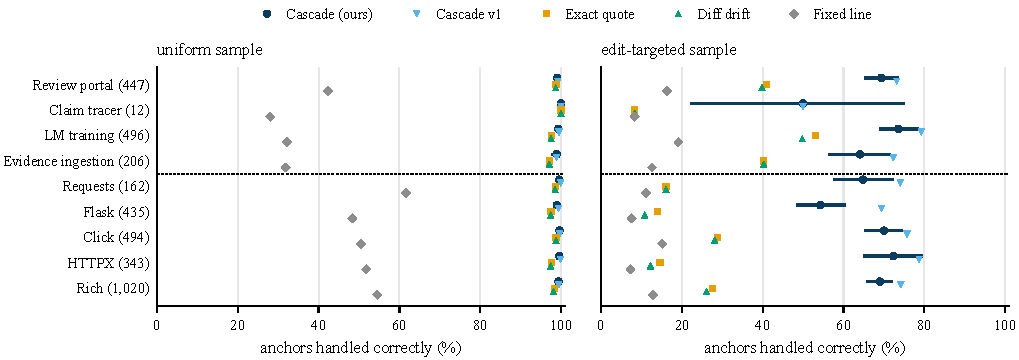
\includegraphics[width=\textwidth]{figures/real-projects-v1.pdf}
\caption{Correct outcome per project on real edit histories (left: uniform sample; right: edit-targeted sample; in brackets the number of edit-targeted anchors). Bars: 95\% bootstrap interval of the cascade over commit pairs. Above the dashed line our projects, below it the open-source ones. The claim tracer has few anchors, hence its wide interval.}
\label{fig:realprojects}
\end{figure*}

\begin{figure*}[t]
\centering
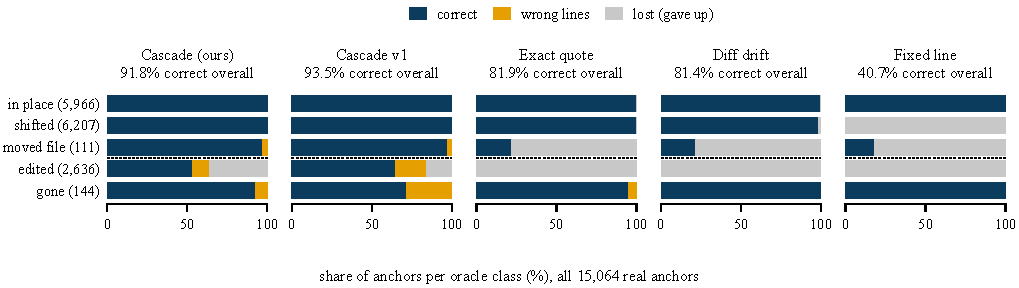
\includegraphics[width=\textwidth]{figures/real-class-v1.pdf}
\caption{Outcome per oracle class for each method on all real anchors, the counterpart of Fig.~\ref{fig:outcomes}. Above the dashed line the anchored content is preserved; below it the content was edited or is gone. Baselines lose every edited anchor; the fixed-line policy also loses every shifted one.}
\label{fig:realclass}
\end{figure*}
On the uniform samples (\rUniformN{} observations), most targets are untouched or shifted and the content-based policies are near the ceiling (Table~\ref{tab:real}). The cascade reaches \rUCas\% pooled over nine projects. Edit-targeting enriches the sample for harder locations without establishing that every selected statement changed: default accuracy is \rOssTCas\% on public projects and \rOwnTCas\% in-house. The cascade leads all three simple policies in each project (Fig.~\ref{fig:realprojects}), but Cascade v1 is stronger at its lower default threshold. Pairwise targeted accuracy is similar across the two sampled horizons (\rTCasHOne\% for adjacent commits and \rTCasHTen\% ten commits apart); this does not test sequential carry.

By reference class (Table~\ref{tab:realclass}, Fig.~\ref{fig:realclass}), the cascade recovers every in-place and shifted target and \rClsMovedFileCas\% of cross-file moves. Its edited-class start recovery is \rClsEditedCas\%, whereas the three simple policies recover none by construction. Fixed lines lose shifted targets, and quote search and diff drift recover only those cross-file moves that Git supplies as renames. These findings establish an advantage over the specified policies on the retained reference set; the independent tracker comparison below tests a stronger within-file alternative.

\begin{figure}[t]
\centering
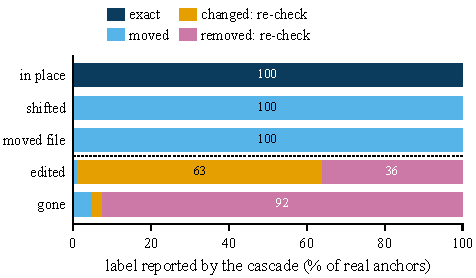
\includegraphics[width=\columnwidth]{figures/real-labels-v1.pdf}
\caption{Label reported by the cascade per oracle class on real edits. Orange and pink labels send the issue back to the supervisor; blue labels keep its state.}
\label{fig:reallabels}
\end{figure}

\subsection{RQ2: Re-checks on Real Edits}
The original score records no cascade silent error among \rN{} retained observations, while diff drift has \rSilentAll{} case. This statement uses the old-height normalized-quote definition. Under that definition, \rNMissed{} of \rNChanged{} changed or gone observations were labelled \lbl{moved} and did not request re-check, giving \rRecall\% recall. No re-check was requested for the \rNPreserved{} preserved-class observations. These values describe label policy, not semantic preservation. The alternative reference analysis below shows why the zero silent-error count cannot support the stronger claim that all changed statements are brought to the supervisor's attention.


\begin{table}[t]
\caption{Quotation Windows and Their Similarity}
\label{tab:realexamples}
\centering
\footnotesize
\tablenote{\begin{tabular}{@{}p{0.86\linewidth}r@{}}\toprule
Original quote and same-height target window & ratio \\ \midrule
{\ttfamily\scriptsize t\_\allowbreak{}hit100 = bench(\allowbreak{}hit\_\allowbreak{}run,\allowbreak{} n=5)} & \\
{\ttfamily\scriptsize t\_\allowbreak{}hit100 = bench(\allowbreak{}hit\_\allowbreak{}run,\allowbreak{} n=7)} & 0.97 \\ \addlinespace
{\ttfamily\scriptsize assert checkpointing[\allowbreak{}"projected\_\allowbreak{}permanent\_\allowbreak{}checkpoint\_\allowbreak{}gib"] < 100.\allowbreak{}0} & \\
{\ttfamily\scriptsize assert checkpointing[\allowbreak{}"projected\_\allowbreak{}remote\_\allowbreak{}permanent\_\allowbreak{}checkpoint\_\allowbreak{}gib"] == 168.\allowbreak{}0} & 0.90 \\ \addlinespace
{\ttfamily\scriptsize results[\allowbreak{}"verify\_\allowbreak{}10k"] = t.\allowbreak{}as\_\allowbreak{}dict(\allowbreak{})} & \\
{\ttfamily\scriptsize results[\allowbreak{}f"verify\_\allowbreak{}\{len(\allowbreak{}rows10k)\}"] = t.\allowbreak{}as\_\allowbreak{}dict(\allowbreak{})} & 0.85 \\ \addlinespace
{\ttfamily\scriptsize self.\allowbreak{}model = Model(\allowbreak{}model\_\allowbreak{}config)} & \\
{\ttfamily\scriptsize self.\allowbreak{}model = Model(\allowbreak{}} & 0.75 \\ \addlinespace
\bottomrule
\end{tabular}}{Ratio: the similarity tier~3 computes between the stripped quotation and the same number of lines at the true location; ratios of at least 0.85 pass the default threshold. Statements from the oracle audit (Appendix~\ref{app:audit}); a class name from a private project is shown generically.}
\end{table}


\subsection{Sensitivity to the Definition of Change}\label{sec:definitionaudit}
The stored rows retain both the oracle's alignment event and the quote-window class. These answer different questions. A statement may expand beyond the old span while leaving the first old-height window unchanged; conversely, reformatting an equal AST statement can change that window. We re-counted the recorded default labels using the oracle's replacement or deletion event as a second reference definition, without rerunning the matcher or changing its threshold (Table~\ref{tab:definitionaudit}).

There are 2,364 same-type AST-replacement observations and 144 deletion observations. Of these 2,508 reference events, 52 were labelled exact or moved and therefore did not request re-check: recall is 97.9\%. Eleven replacement observations were labelled exact. Twenty-one replacements were classified as preserved by the original window definition (11 exact and 10 moved). In the other direction, 293 aligned equal-tree observations were classified edited because the quote window differed. The two denominators are not nested, so the 97.9\% and 98.7\% rates must not be subtracted as a paired performance improvement.

This is a sensitivity analysis of the same retained observations, including repeats. The oracle's replacement marker is not a human judgement of semantic relevance and can itself contain pairing errors. Nevertheless, the disagreement is sufficient to bound the original interpretation: zero errors under a quote-window definition does not establish that no structural statement change was labelled exact. The no-auto-resolution invariant remains separate from both matching metrics.

\begin{table}[t]
\caption{Re-check Recall Under Two Reference Definitions}
\label{tab:definitionaudit}
\centering\footnotesize
\begin{tabular}{@{}lrrrr@{}}\toprule
Reference definition & $n$ & Missed & Exact & Recall \\
\midrule
Quote window changed / gone & 2,780 & 37 & 0 & 98.7\% \\
AST replacement / deletion & 2,508 & 52 & 11 & 97.9\% \\
\bottomrule
\end{tabular}
\par\smallskip
\parbox{\columnwidth}{\scriptsize Same 15,064 retained observations and default cascade; the denominators select different reference events. Missed means labelled exact or moved, neither of which requests re-check. Exact is the number of misses labelled exact. The AST row uses the oracle's replacement/deletion marker and is a sensitivity analysis, not a human semantic judgement. Repeated observations are retained to match the original analysis.}
\end{table}


\subsection{Verification Against Complete Source Revisions}\label{sec:sourcecontext}
Saved quotations alone cannot establish whether a reference points into the correct revision. We recovered the recorded heads of all nine histories and reconstructed each pair from its first-parent index and horizon. The five public heads were fetched at their recorded revisions with depth 400. Their first-parent counts matched the archive: 626, 448, 589, 400 and 1,093. Full head identifiers, traversal lists, shallow boundaries, pair revisions and file hashes are retained in the verification artifact. Private source remained local. No project source was executed.

We separately reran the original sampling and AST-reference procedure from the pinned histories, omitting only matcher evaluation and timing. In-house repositories used the original shared random stream and order; each separately collected public repository restarted seed 20261028. All 15,064 ordered retained observations matched the saved selection, source coordinates, quotation text and reference class. The 2,205 exclusions and every per-project exclusion-reason count also matched. This verifies deterministic regeneration under Python 3.12.14, not independent human validity of the reference rule. The retained per-project reports distinguish this check from the complete-source coordinate check and the saved-row aggregation.

All 15,064 old quotations matched the reconstructed old revision. Every assigned reference's saved old-height target window also matched the new revision. For 14,917 non-deleted observations, the old and referenced new function-body statements could be uniquely recovered and compared structurally: all 2,364 replacement markers had different syntax trees, while the 12,553 aligned/relocated markers had equal trees. Three further observations had ambiguous same-line statement extraction in this additional checker; 144 had no assigned surviving target. These checks validate recorded coordinates and structural relations. They do not establish that a same-type replacement is the same conceptual entity, independently prove deletion, or replace human adjudication.

The complete source explains the 21 observations where the quote window is preserved but the reference statement changes. Nineteen observations (18 distinct pair/anchor targets) grow beyond the old range. The remaining two change decorators above a function definition, outside the line interval the original AST-based sampler used. Together these are 20 distinct targets, since one growing target occurs in both sampling schemes. Eleven observations retain an exact label: ten growing statements and one decorator change. The other ten are labelled moved. These are concrete limits of the quoted interval, rather than evidence that every such change violates the matcher's normalized-text contract.

For example, a Click revision renames the decorator call from \texttt{resultcallback} to \texttt{result\_callback} above an otherwise unchanged function \cite{clickdecoratorcase}. The AST includes the decorator; the sampled quote begins at the function's definition line and omits it. The exact label is therefore compatible with identical quoted lines, but cannot certify an unchanged complete statement. Similarly, retaining the old number of lines omits a growing statement's new suffix. These examples motivate evaluating complete source extents and relevant context separately from quote preservation.

We also prepared a source-based review packet with expected targets and matcher outcomes withheld. It contains 50 cases stratified equally across the original five reference classes and the 20 distinct quote/AST disagreements, shuffled in a recorded order. The unblinding key is separate. No independent reviewer responses have been collected, so the packet is preparation for validation, not a human-validation result.

\subsection{RQ3: Real-Edit Trade-offs}
\begin{figure*}[t]
\centering
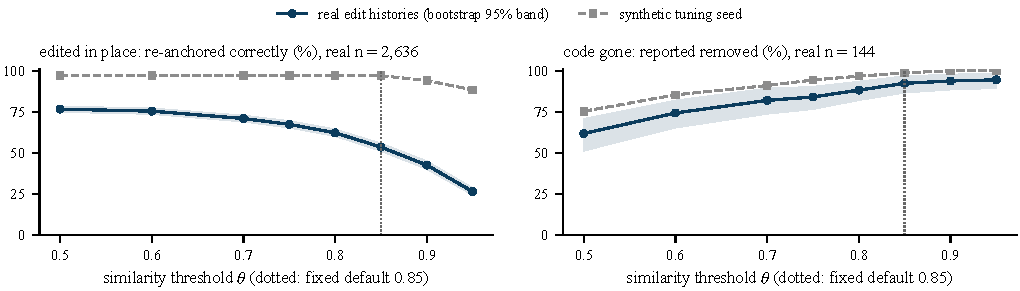
\includegraphics[width=\textwidth]{figures/real-theta-v1.pdf}
\caption{Fuzzy-tier threshold on real edits (solid, with 95\% bootstrap band over commit pairs) against the synthetic tuning seed of Fig.~\ref{fig:threshold} (dashed). Left: edited statements re-anchored correctly. Right: gone statements correctly reported \lbl{removed}. The method keeps the fixed-default $\theta=0.85$ (dotted).}
\label{fig:realtheta}
\end{figure*}
Real edits are more varied than single-identifier mutations: calls expand, arguments change and statements are reformatted. Table~\ref{tab:realexamples} illustrates the similarity calculation on recorded windows, which may truncate a growing statement. At $\theta=0.85$, only \rClsEditedCas\% of edited-class observations are placed at the reference start. Many others return removed and therefore request re-check, but the effect on a reviewer's time or judgement was not measured. Gone targets account for only \rGoneN{} retained real observations, compared with a sixth of the controlled trials. This selected distribution explains why the default v1 comparator, with a lower threshold and wider search, leads on real edit-targeted accuracy by \rTVoneLead{} points (95\% CI \rTVoneLeadLo--\rTVoneLeadHi), while identifying fewer gone targets correctly (\rClsGoneVone\% versus \rClsGoneCas\%). It does not establish deletion prevalence in student review. Fig.~\ref{fig:realtheta} shows the final cascade's threshold trade-off: at $\theta=0.7$, edited-class start recovery is \rThetaEdSeventy\% and gone-target removal detection is \rThetaGoneSeventy\%. Calibration should therefore report both outcomes and validate the reference labels.

% Held-out threshold calibration (shared by both papers; numbers from analyse_real.py).
\subsection{Held-Out Threshold Calibration}\label{sec:calibration}
We selected a threshold on all anchors of the four in-house projects and reported its result on the five public projects. Selection maximized correct start-location outcomes, with ties favoring the stricter value. This is project-disjoint calibration: public-project rows are not part of the selection objective. The analysis is secondary to the default comparison, and no dated prospective holdout protocol is established. Maximizing aggregate correctness also weights edit and deletion errors by their frequency in the choosing set, rather than by a measured cost to reviewers.

\begin{figure}[t]
\centering
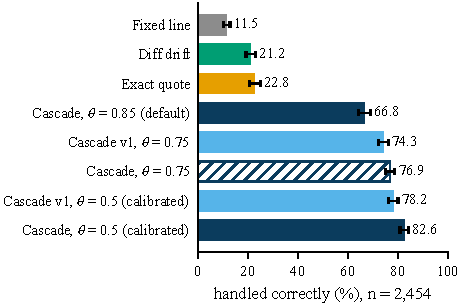
\includegraphics[width=\columnwidth]{figures/real-heldout-v1.pdf}
\caption{Held-out calibration on the open-source edit-targeted sample, with 95\% bootstrap intervals over commit pairs. The calibrated threshold was chosen on our four projects only. Hatched: the final design at Cascade v1's threshold; threshold is held equal while window scope and tier order still differ.}
\label{fig:heldout}
\end{figure}

\textbf{Choice.} On our projects the best value was $\theta=\rCalTheta$, which handled \rCalOwnAll\% of their anchors correctly against \rCalOwnAllPre\% at 0.85. It is the lowest value of the grid we evaluated, so a lower optimum cannot be ruled out.

\textbf{Held-out result.} On the open-source edit-targeted sample the calibrated cascade reached \rCalOssTCas\% [\rCalOssTCasLo, \rCalOssTCasHi] (Fig.~\ref{fig:heldout}), ahead of Cascade v1 by \rCalOssTVoneD{} points (95\% CI \rCalOssTVoneDLo--\rCalOssTVoneDHi), and the uniform sample stayed at \rCalOssUCas\%. Edited statements re-anchored correctly rose from \rCalOssEditedPre\% to \rCalOssEdited\%. The price is paid on deleted code: of the \rCalOssGoneN{} gone anchors, \rCalOssGone\% were reported \lab{removed}, against \rCalOssGonePre\% at 0.85 and \rCalOssGoneVone\% for Cascade v1; the rest were attached to similar nearby lines. Preserved anchors were handled correctly in \rCalOssPres\% of cases (\rCalOssPresPre\% at 0.85).

\textbf{Effect on label policy.} Lowering $\theta$ only changes tier~3, which never reports \lab{exact}, so it cannot add an exact-label error through that tier under the original scoring definition. Tier~3 also runs before tier~4: an anchor it now accepts was previously reported \lab{removed}, which already asked for a re-check, or \lab{moved} to an identical copy, which did not. Under the stated tier order, lowering the threshold does not remove an existing changed/removed re-check flag; it can still produce an incorrect location. It can add unnecessary ones, when a preserved block that moved to another file is matched to similar lines near its old place.

\textbf{Equal thresholds.} The comparison with Cascade v1 is fairest at an equal threshold. With $\theta=0.75$ for both, the final design was ahead by \rEqOssTD{} points on the open-source edit-targeted sample (\rEqOssTCas\% against \rEqOssTVone\%, CI \rEqOssTDLo--\rEqOssTDHi) and by \rEqOwnTD{} points on ours (CI \rEqOwnTDLo--\rEqOwnTDHi). The ordering at the unequal default settings therefore reverses when thresholds are held equal. This supports the final combined search policy on this retained sample, but does not identify separate effects of window scope and tier order. A course-specific threshold would require representative review anchors and explicit error costs.

\begin{figure*}[t]
\centering
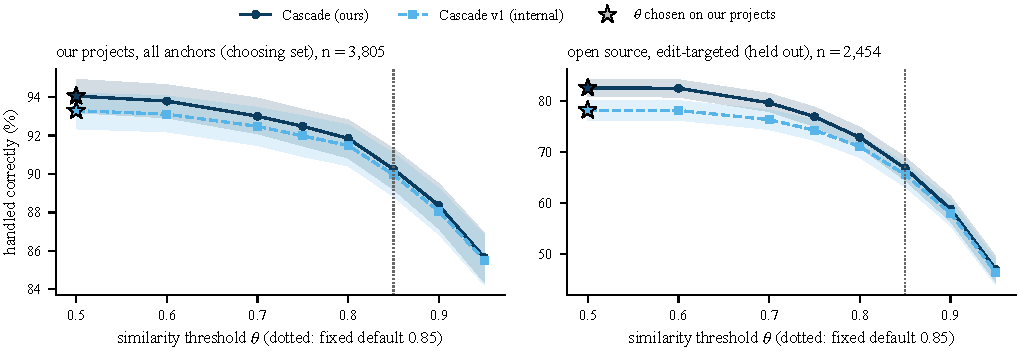
\includegraphics[width=\textwidth]{figures/real-v1theta-v1.pdf}
\caption{Final cascade and internal comparator (Cascade v1) across the threshold grid, with 95\% bootstrap bands over commit pairs. Left: our projects, where each design's threshold is chosen (stars). Right: the held-out open-source edit-targeted sample. Point estimates favor the final design at every threshold; panels use different vertical scales.}
\label{fig:v1theta}
\end{figure*}

\textbf{Each design at its own best threshold.} Cascade v1 might gain as much from calibration as the final design, so we chose its threshold the same way, on our projects only. Its best value was also $\theta=\rBestVoneTheta$ (\rBestVoneOwnAll\% of our anchors correct, against \rCalOwnAll\% for the final design). On the held-out open-source edit-targeted sample calibrated Cascade v1 reached \rBestVoneOssT\%, and the calibrated final design was ahead by \rBestD{} points (95\% CI \rBestDLo--\rBestDHi). The final design led at every threshold of the grid, on our projects and on the held-out ones (Fig.~\ref{fig:v1theta}, Table~\ref{tab:realbest}). The difference is largest on deleted code: at its calibrated threshold Cascade v1 reported only \rBestVoneOssGone\% of gone open-source anchors as \lab{removed}, against \rCalOssGone\% for the final design, consistent with its broader search accepting distant look-alike lines. Neither design made an exact-label error under the original quote-window score at any tested threshold; this does not establish complete structural change detection.


\subsection{Independent Tracker on Real Histories}\label{sec:realtracker}
We extended the pinned hybrid tracker from Section~\ref{sec:externaltracker} to the same 15,064 retained real-history observations. The input is the complete old file and its corresponding new path, using Git rename detection as for the original simple policies. The reference target path is never supplied as a search hint. Mapping the old anchor's first line gives a candidate start; scoring retains the original file/start reference. Thus this experiment compares location recovery, not the review-state policy or complete returned ranges. It remains conditional on the original oracle and exclusions.

The unmodified tracker dependency crashes on some non-BMP Unicode characters: its Levenshtein implementation indexes a 65,536-element table with a larger code point. We reproduced that failure with a minimal changed emoji line. A failed process is discarded before another file pair is evaluated, preventing partially mutated global state from affecting later requests. Neither source text nor the matching algorithm is patched. Failed file pairs are recorded as execution errors, not silently removed or relabelled as a successful no-match. The run completes with 143 affected observations across 37 distinct source-content file pairs, all in the public group. The 143 observations comprise 85 uniform and 58 edit-targeted cases. A regression check confirms both explicit failure reporting and a fresh successful request afterward.

\begin{table*}[t]
\caption{Independent Tracker on Retained Real-History Observations}\label{tab:realtracker}
\centering\small
\begin{tabular}{@{}llrrrr@{}}\toprule
Project group & Sample & $n$ & Tracker correct \% [95\% CI] & Execution errors & Cascade default / calibrated \% \\
\midrule
In-house & uniform & 2,644 & 99.5 [98.9, 99.9] & 0 & 99.1 / 99.4 \\
In-house & edit-targeted & 1,161 & 89.8 [87.4, 92.1] & 0 & 70.0 / 81.8 \\
Public & uniform & 8,805 & 98.7 [98.2, 99.1] & 85 & 99.4 / 99.7 \\
Public & edit-targeted & 2,454 & 83.6 [81.6, 85.5] & 58 & 66.8 / 82.6 \\
\bottomrule
\end{tabular}
\par\smallskip
\parbox{.97\textwidth}{\footnotesize Correct percentages use all retained observations; an execution error contributes no correct location. Intervals are 2,000 percentile bootstrap resamples of commit pairs, seed 20261028. Calibration is the existing 0.5 setting chosen on in-house observations; the independent tracker uses its unchanged defaults. On completed public observations alone, tracker accuracy is 99.6\% for uniform and 85.6\% for edit-targeted cases. These conditional figures describe a different subset, so paired comparisons must restrict both methods to that same subset.}
\end{table*}

The tracker correctly locates 1,043 of 1,161 in-house edit-targeted observations (89.8\%) and 2,052 of 2,454 public edit-targeted observations (83.6\%, including execution failures in the denominator). The default cascade reaches 70.0\% and 66.8\%, respectively. On public edit-targeted observations the default cascade-minus-tracker difference is $-16.8$ percentage points, with a commit-pair interval of $[-19.3,-14.4]$. This reverses any interpretation that the cascade's advantage over simple policies establishes generally stronger within-file tracking.

Calibration narrows the public edit-targeted gap: 82.6\% for the cascade versus 83.6\% for the tracker. Their paired difference is $-1.0$ point, interval $[-3.1,1.1]$; this analysis does not resolve its direction and is not an equivalence test. On the 2,396 public edit-targeted observations where the tracker completes, its accuracy is 85.6\%, compared with 82.2\% for the calibrated cascade on that same subset. Failures and conditional accuracy therefore need separate reporting. The in-house edit-targeted sample has no tracker execution failures and still favors the tracker over both cascade settings.

By original reference class, the tracker correctly handles 2,192 of 2,636 edited observations (83.2\%), including 51 execution errors as unsuccessful outcomes, versus 1,412 (53.6\%) for the default cascade. The cascade is stronger on the 111 cross-file observations (108 correct versus 25, largely those available through Git renames) and on 144 gone targets (133 versus 122). The comparison supports distinct engineering choices: stronger within-file localization is available, while cross-file recovery, removal conservatism and implementation robustness matter separately. Keeping persistent issue state independent of the chosen tracker allows that component to be evaluated or replaced without treating a recovered location as proof of resolution.


\subsection{RQ1: Source-Line Range Recovery}\label{sec:ranges}
The original location metric checks the reference file and start, not the returned end line. We ran the pinned cascade again at the unchanged default and previously calibrated thresholds on every retained observation, using the complete new-version Python file map and previous file. All 15,064 default labels and both thresholds' path/start outcomes matched the saved records. A local exploratory protocol preceded this run; it was not externally registered. No threshold was tuned for the new metric.

The primary denominator is the 14,917 surviving observations whose old and referenced new statements were uniquely recovered in Section~\ref{sec:sourcecontext}. An exact range must match the reference file, start and the new AST node's inclusive \texttt{end\_lineno}. We exclude the three ambiguous same-line extractions from both thresholds' range metrics. The 144 gone observations remain a separate removal outcome: 133 correctly reported removed at the default threshold and 89 at the calibrated value. This AST line extent is a syntactic proxy, not a validated boundary of the review concern; decorators above the definition and other relevant context remain outside it.

\begin{table*}[t]
\caption{Start and Exact Source-Line Range Accuracy on the Same Surviving Targets}\label{tab:ranges}
\centering\small
\begin{tabular}{@{}llrrrrr@{}}\toprule
& & & \multicolumn{2}{c}{Default $\theta=0.85$} & \multicolumn{2}{c}{Calibrated $\theta=0.5$} \\
Project group & Sample & $n$ & File/start \% & File/start/end \% & File/start \% & File/start/end \% \\
\midrule
In-house & uniform & 2,636 & 99.1 & 98.9 & 99.4 & 99.0 \\
In-house & edit-targeted & 1,136 & 69.7 & 63.3 & 82.1 & 70.8 \\
Public & uniform & 8,786 & 99.4 & 99.3 & 99.7 & 99.6 \\
Public & edit-targeted & 2,359 & 65.8 & 62.0 & 83.7 & 76.8 \\
\bottomrule
\end{tabular}
\par\smallskip
\parbox{.97\textwidth}{\footnotesize Both metrics in each row use exactly the same surviving observations. Three ambiguous AST extractions and 144 gone targets are outside this table. Complete returned coordinates are retained. The line-only external tracker has no statement-range policy and is not assigned an invented end line.}
\end{table*}

On the 2,359 surviving public edit-targeted observations, calibrated accuracy falls from 83.7\% for file/start to 76.8\% for the exact range (Table~\ref{tab:ranges}). The paired reduction is 6.9 percentage points, with a 95\% commit-pair bootstrap interval of $[5.8,7.9]$. The default falls from 65.8\% to 62.0\%, a 3.8-point reduction, interval $[3.0,4.6]$. These intervals use 2,000 paired resamples, seed 20261028, with the same pair-cluster/percentile convention as the other real-history analyses. The denominators differ from the original all-target accuracy because gone targets are not assigned a surviving range.

The boundary limitation is concentrated in changed line spans. Of 824 observations whose new reference span differs from the original height, only four have exact ranges at either threshold. The default finds 182 correct starts in this subset, but 165 ranges truncate the statement and 13 extend beyond it; calibration finds 321 correct starts, with 274 truncated and 43 extended ranges. Across all 14,917 surviving observations, start/range accuracy is 91.8\%/90.6\% at default and 95.8\%/93.7\% after calibration. Within the original edited class, the corresponding exact-range figures are 47.6\% and 65.3\% on 2,634 recoverable observations. These are conditional benchmark results, not estimates of classroom prevalence.

The mechanism explains the result: the fuzzy tier preserves the old window height, while exact normalized runs can span blank-line changes. Lowering the similarity threshold recovers more starts, but does not adapt the end boundary to a growing or shrinking statement. Mean line-interval intersection-over-union across surviving targets is 0.923 at default and 0.967 after calibration; overlap can therefore improve without exact boundaries. Recovering a usable location, recovering the complete syntactic extent, and deciding whether a concern is resolved remain separate tasks.


\subsection{RQ5: Ten Successive Revision Hops}\label{sec:chains}
Pairwise relocation does not test the effect of carrying an updated anchor repeatedly. We replayed all 4,000 original horizon-10 observations across their intervening first-parent commits: 367 intervals and 3,959 distinct interval/anchor-start targets, retaining repeated samples. Each comparison uses the same initial anchor, final revision and archived endpoint reference. The direct route makes one initial-to-final call; the sequential route invokes the pinned code-anchor carry function ten times, feeding its returned quote, digest and coordinates into the next hop with the actual previous file map. Both thresholds are unchanged. Direct labels, outcomes and coordinates reproduce the archived and range-run evidence. Intermediate no-match results do not stop or exclude a chain. A local exploratory protocol preceded execution; it was not externally registered.

\begin{table*}[t]
\caption{Endpoint File/Start Accuracy: Direct Relocation Versus Ten Successive Carries}\label{tab:chains}
\centering\small
\begin{tabular}{@{}llrrrrr@{}}\toprule
& & & \multicolumn{2}{c}{Default $\theta=0.85$} & \multicolumn{2}{c}{Previously calibrated $\theta=0.5$} \\
Project group & Sample & $n$ & Direct \% & Ten-hop \% & Direct \% & Ten-hop \% \\
\midrule
In-house & uniform & 503 & 99.0 & 99.0 & 99.6 & 99.6 \\
In-house & edit-targeted & 292 & 69.5 & 70.2 & 82.2 & 83.2 \\
Public & uniform & 2,228 & 99.5 & 99.5 & 99.6 & 99.6 \\
Public & edit-targeted & 977 & 66.7 & 67.1 & 82.9 & 83.1 \\
\bottomrule
\end{tabular}
\par\smallskip
\parbox{.97\textwidth}{\footnotesize Each row compares routes on the same original-to-final endpoint references, including correct no-match for gone targets. All 39 gone endpoint references are retained. Intermediate identity is not independently labelled; these are Git-history replays, not observed student resubmissions.}
\end{table*}

Endpoint accuracy changes little in this selected sample (Table~\ref{tab:chains}). At default, 3,569 observations are correct directly and 3,575 sequentially: eight become correct and two become incorrect. At the previously calibrated threshold, the counts are 3,770 and 3,775: eight gains and three losses. On public edit-targeted observations, the sequential-minus-direct differences are 0.4 points, 95\% interval $[-0.2,1.1]$, and 0.2 points, interval $[-0.4,0.9]$, respectively. Intervals use 2,000 paired commit-interval resamples, seed 20261028. No equivalence margin was specified, so small net changes do not establish drift-free operation. Exact-range correctness on the 3,961 eligible surviving endpoints increases by only three observations at default and one after calibration.

The trace labels expose a different question from endpoint accuracy. At default, 82 endpoint errors end with an exact last-hop label; 74 of these have an earlier changed/removed request. After calibration, 188 errors end exact and 184 have an earlier request. Under an explicit no-faculty-action simulation, the OR of all requests therefore preserves information that the latest label alone omits. It is not complete protection: ten default endpoint errors and five calibrated errors have no re-check request anywhere in the chain. These counts are neither new semantic-error labels nor faculty workload estimates, and the replay does not exercise database lifecycle or human decisions.

A source-checked Flask trace illustrates the mechanism \cite{flaskchaincase}. Its original negative assertion is present at line 491 in both endpoint revisions. At hop 7, fuzzy matching selects a nearby positive assertion and replaces the stored quote; when the negative assertion returns, the updated quote follows the positive one to line 494 and later receives exact labels. Direct relocation finds line 491. The earlier re-check request is retained by the cumulative indicator, but the final local exact label cannot certify the original referent. This is a diagnostic example selected after the comparison, not independent adjudication of every intermediate identity. The complete revisions, output coordinates and quote hashes are retained.

\section{Threats to Validity}
\label{sec:threats}

\subsection{Construct Validity}
The synthetic edit mix is uniform and includes source mutations that need not remain valid Python. The original start metric is separate from the additional AST-line range metric in Section~\ref{sec:ranges}. Neither establishes semantic equivalence or continued relevance of a comment. Unique-quotation and minimum-length restrictions exclude common ambiguous anchors. An old-height window can miss growth in a statement; the reference-definition analysis quantifies this limitation in retained rows. Changes outside the quoted range can also matter to the concern, and are not systematically evaluated.

\subsection{Oracle Validity}
The oracle samples statements directly in function bodies, excluding module-level code and class attributes. It excludes \rExcludedPct\% of candidate observations, disproportionately difficult rewrites and duplicate targets. Accuracy is conditional on that decidable subset. Equal-cardinality same-type pairing is heuristic, and the small in-house audit includes one doubtful pairing. Its direction of bias is not necessarily conservative for every method. Independent blinded annotation of public, excluded and rare-class cases is needed before treating the oracle as a gold standard.

\subsection{Internal Validity}
The fixed default was selected using a separate synthetic seed, while calibration uses a project-disjoint secondary split. No externally registered protocol is documented. Policy baselines omit capabilities of full tools. The default internal comparator changes three choices together; equal-threshold comparisons still combine order and scope. Repeated targets and temporal overlap limit pair-level inference. Real-history intervals and calibration outputs can be regenerated from the retained rows, but regenerating rows requires the exact source histories and matcher snapshot.

\subsection{External Validity}
The real histories add five widely used Python libraries to four in-house projects, but neither group consists of faculty-selected student review anchors. The two commit horizons are not measured proxies for student resubmissions. All sampled files are Python; operating on arbitrary text does not establish equal performance across languages, prose or PDFs. The ten-hop replay in Section~\ref{sec:chains} measures endpoint outcomes across selected commit chains, but lacks independently labelled intermediate identities or human interventions. It does not validate longer chains or student resubmissions.

\subsection{Scope}
The experiments measure code-anchor start locations, label-derived re-checks, AST line extents and ten-hop endpoint outcomes on explicitly defined samples. Report anchors, media accessibility, permission checks, dismissal matching and concurrent composition have separate integration requirements. Faculty workload, student engagement, resolution correctness and educational outcomes remain unmeasured.

% Appendix tables (shared by both papers), input before the discussion so they float ahead of the references.


% Discussion (shared by both papers).
\section{Discussion}\label{sec:discussion}

\subsection{Why Carrying Content Works}
Content enables the cascade to recover many shifted and edited targets that the simple policies decline to place. The useful workflow property is that a failed relocation retains the concern and requests re-check rather than resolving it. That property does not establish the cost of a failed or incorrect match: a plausible wrong attachment can misdirect review, and a moved label can suppress re-check. Faculty should be able to inspect both the original quotation and its earlier context alongside the proposed location.

\subsection{How Strong Is the Method?}
The answer depends on the target population, reference definition and threshold. The 98.5\% synthetic result measures a balanced controlled edit mix. The 67.8\% real edit-targeted result includes preserved statements overlapping a diff hunk and is lower than the internal comparator at its default. At equal calibrated thresholds, the final cascade leads that comparator by 4.4 points on the public edit-targeted sample, but removal detection worsens. Re-check recall is 98.7\% for quote-window changes and 97.9\% for the oracle's replacement/deletion events. The independent tracker leads within-file controlled matching and default-cascade edit-targeted real-history localization (Sections~\ref{sec:externaltracker} and~\ref{sec:realtracker}). These findings bound the integration rather than establish universal matching superiority or safety.

\subsection{Deploying the Method in a Course}
The results suggest evaluating thresholds against local revision patterns and the cost of wrong attachments, rather than adopting the accuracy-maximizing value automatically. A conservative threshold detects more gone targets as removed; a lower value recovers more edited starts while accepting more substitutes for deleted code. Preserve explicit labels, earlier context and human resolution regardless of threshold. Before classroom claims, a consented task study should measure correct judgements, missed concerns, erroneous closure and time. The current per-anchor timings do not establish workload savings.

\subsection{Ethics and Data Handling}
No student submission was used in this evaluation. The synthetic benchmark used our own project code, and the real histories came from our projects and from public open-source repositories, which were parsed and never executed. In the portal, feedback stays private to the supervisors until it is shared, and a student sees only the frozen packet addressed to them. Research telemetry in the portal is separate from course access: it requires opt-in consent, synthetic demonstration data are excluded from research aggregates, and declining consent does not change a student's access to the course. A classroom study would require institutional approval and an appropriate consent process.

\subsection{Future Work}
Priority experiments are additional canonical source-tracking implementations and independent oracle annotation covering public and excluded cases; range-adaptive recovery and human validation of concern boundaries; duplicate/context-change stress tests; and longer chains with independently labelled identities and actual reviewer interventions. A factorial comparison is needed to separate window scope from tier order. A classroom study can then test whether persistent anchors improve review judgements and effort. These experiments require new evidence; the present analysis does not supply their outcomes.


\section{Conclusion}
\sys{} connects content-based relocation to persistent review state. Controlled edits show high start-location accuracy, with the aggregate gain over an independent tracker coming from cross-file scope; real histories expose lower edited-target recovery and a material threshold trade-off. Project-disjoint calibration improves public edit-targeted accuracy while reducing correct removal detection. Complete-source checks confirm AST replacements labelled exact despite zero errors under the quote-window metric, while an independent tracker outperforms the default cascade on real edit-targeted locations. Exact source-line extent recovery is lower than start accuracy and is particularly limited when a statement changes height. Ten-hop replay shows why earlier requests must remain visible alongside the latest local label. The lifecycle reserves resolution for faculty, but the matcher does not guarantee semantic preservation or complete change detection. The contribution is an implementable integration and a bounded empirical characterization, with independent oracle adjudication, additional tracking implementations and faculty evaluation still required.

\section*{Acknowledgment}
OpenAI Codex \cite{openaicodex} assisted with substantial prose revision in the Abstract, Sections I--X, Reproducibility and Appendices A--E; preparation of reproduction and comparison code; source-history reconstruction; numerical cross-checks; and bibliographic and primary-source claim checking. The added complete-source, reference-definition, range-boundary, revision-chain and independent-tracker analyses were developed with this assistance and are distinguished from the original archived experiments. The artifact retains the executed code and numerical outputs; independent human reference adjudication remains open.

\section*{Reproducibility}
The research archive contains the controlled benchmark summaries, both real-history row files, threshold outcomes, analysis scripts, figures and a 40-case oracle audit. The synthetic corpus and four in-house histories are private. The corpus is pinned separately from the current application, and its recorded 117-file, 32,446-line inventory is recoverable from those revisions. A complete reviewer artifact must provide the permitted source snapshots or access procedure, exact full revision mapping, environment and commands. Local availability does not imply a public artifact or reviewer access permission.

The public-project heads are recorded as Requests \texttt{3c7baaa}, Flask \texttt{d086db8}, Click \texttt{2247b35}, HTTPX \texttt{b5addb6}, and Rich \texttt{9d8f9a3}. Exact history traversal and shallow boundaries must accompany a source-history regeneration. The original synthetic JSON retains summaries rather than trial rows. Re-exporting the pinned corpus and rerunning both seeds reproduced every non-timing summary field and retained 7,200 individual observations. Timing agreement is not required across environments. The real-history files retain individual observations and threshold outcomes. Re-aggregation reproduced all six numerical table/macro files; selection-only regeneration separately reproduced the ordered references and exclusions. The added complete-source, reference-definition, range, chain and independent-tracker analyses are identified separately from the archived experiments. No student code or source project needs to be executed for these analyses.

\appendices
% Appendix sections (shared by both papers); each paper starts its own appendix before this input.

\section{Per-Project Results}\label{app:projects}
\begin{table*}[t]
\caption{Real-History Study per Project}
\label{tab:projects}
\centering
\footnotesize
\tablenote{\begin{tabular}{@{}lrrrrcccccc@{}}\toprule
 & & & & & uniform & \multicolumn{5}{c}{edit-targeted (correct \%)} \\ \cmidrule(lr){7-11}
Project & commits & authors & pairs & anchors & cascade & cascade & v1 & quote & drift & line \\ \midrule
Review portal & 444 & 3 & 193 & 1,584 & 99.0 & 69.4 & 73.2 & 40.9 & 39.8 & 16.3 \\
Claim tracer & 40 & 2 & 18 & 87 & 100.0 & 50.0 & 50.0 & 8.3 & 8.3 & 8.3 \\
LM training & 203 & 2 & 168 & 1,476 & 99.3 & 73.6 & 79.2 & 53.0 & 49.8 & 19.2 \\
Evidence ingestion & 108 & 2 & 78 & 658 & 98.9 & 64.1 & 72.3 & 40.3 & 40.3 & 12.6 \\
\midrule
Requests & 626 & 240 & 229 & 1,260 & 99.5 & 64.8 & 74.1 & 16.0 & 16.0 & 11.1 \\
Flask & 448 & 179 & 245 & 1,792 & 99.0 & 54.3 & 69.4 & 14.0 & 10.8 & 7.6 \\
Click & 589 & 240 & 331 & 2,359 & 99.6 & 70.0 & 75.7 & 28.7 & 28.1 & 15.2 \\
HTTPX & 400 & 104 & 187 & 1,409 & 99.5 & 72.3 & 78.7 & 14.6 & 12.2 & 7.3 \\
Rich & 1,093 & 273 & 624 & 4,439 & 99.4 & 69.0 & 74.2 & 27.5 & 26.1 & 12.8 \\
\bottomrule
\end{tabular}}{Uniform: cascade, correct \%. Edit-targeted: correct \% of each method. Above the rule our projects, below it the open-source ones (shallow clones of the default branch, depth 400).}
\end{table*}
Table~\ref{tab:projects} lists each project of the real-history study with the number of first-parent commits, contributors (distinct author names), commit pairs and decidable anchors, and the correct outcome of each method on the edit-targeted sample. The claim tracer contributes few anchors because its history is short.

\section{Threshold Sensitivity on Real Edits}\label{app:theta}
\begin{table}[t]
\caption{Final Cascade and Internal Comparator Across Thresholds}
\label{tab:realbest}
\centering
\footnotesize
\tablenote{\begin{tabular}{@{}lcccc@{}}\toprule
 & \multicolumn{2}{c}{ours, all anchors} & \multicolumn{2}{c}{open source, edit-targeted} \\ \cmidrule(lr){2-3}\cmidrule(l){4-5}
$\theta$ & cascade & v1 & cascade & v1 \\ \midrule
0.5 & 94.1 & 93.3 & 82.6 & 78.2 \\
0.6 & 93.8 & 93.1 & 82.5 & 78.2 \\
0.7 & 93.0 & 92.5 & 79.7 & 76.4 \\
0.75 & 92.5 & 92.0 & 76.9 & 74.3 \\
0.8 & 91.9 & 91.5 & 72.9 & 71.1 \\
0.85 & 90.2 & 90.0 & 66.8 & 65.6 \\
0.9 & 88.4 & 88.1 & 58.8 & 58.0 \\
0.95 & 85.7 & 85.5 & 46.9 & 46.3 \\
\bottomrule
\end{tabular}}{Correct outcome (\%). Left: all anchors of our four projects, the set on which each design's threshold is chosen. Right: the held-out open-source edit-targeted sample. Both designs select 0.5 on the choosing set.}
\end{table}

\begin{table}[t]
\caption{Fuzzy-Tier Threshold on Real Edits}
\label{tab:realtheta}
\centering
\footnotesize
\tablenote{\begin{tabular}{@{}lccc@{}}\toprule
$\theta$ & edited: re-anchored & gone: reported removed & all anchors \\ \midrule
0.5 & 76.6 & 61.8 & 95.5 \\
0.6 & 75.4 & 74.3 & 95.4 \\
0.7 & 70.9 & 81.9 & 94.7 \\
0.75 & 67.4 & 84.0 & 94.1 \\
0.8 & 62.3 & 88.2 & 93.3 \\
0.85 & 53.6 & 92.4 & 91.8 \\
0.9 & 42.6 & 93.8 & 89.9 \\
0.95 & 26.5 & 94.4 & 87.1 \\
\bottomrule
\end{tabular}}{Every column is the final cascade; the columns are kinds of code, not methods. Correct outcome (\%) on edited statements, on deleted statements and on all real anchors. The method uses the fixed-default 0.85; gone code has only \rGoneN{} cases. Table~\ref{tab:realbest} compares Cascade v1 across the same thresholds (Appendix~\ref{app:theta}).}
\end{table}
Table~\ref{tab:realtheta} gives the values plotted in Fig.~\ref{fig:realtheta}, together with the share of all real anchors handled correctly at each threshold. Only the approximate tier depends on $\theta$. Anchors settled by tiers~1 and~2 (untouched and shifted code) are therefore handled identically in every row; only anchors that reach tier~3 (edited and gone code, and code moved to another file) can change.

\section{Oracle Audit}\label{app:audit}
The recorded audit draws 40 in-house observations with seed 7: 20 from edited, gone and moved-file classes, and 20 from preserved classes. The file \texttt{oracle-audit-v1.txt} records the compared quotations and judgements. Thirty-nine decisions were accepted; one pairing of unrelated same-type statements was marked doubtful. These are the recorded audit judgements, not an independent multi-rater validation. The sample does not establish accuracy on public-project, excluded or rare-class observations, and the direction of reference error need not favor or penalize every matcher equally.

\section{Reproducing the Results}\label{app:repro}
\begin{table*}[t]
\caption{Correct Outcome (\%) per Edit Type, \nPerOp{} Trials Each, Seed \seedMain}
\label{tab:pertype}
\centering
\small
\tablenote{\begin{tabular}{@{}lccccc@{}}\toprule
Edit type & Cascade (ours) & Cascade v1 & Exact quote & Diff drift & Fixed line \\ \midrule
no change & 100.0 & 100.0 & 100.0 & 100.0 & 100.0 \\
edit elsewhere & 100.0 & 100.0 & 100.0 & 100.0 & 100.0 \\
insert above & 100.0 & 100.0 & 100.0 & 100.0 & 0.0 \\
delete above & 100.0 & 100.0 & 100.0 & 100.0 & 0.0 \\
re-indent & 100.0 & 100.0 & 100.0 & 0.0 & 100.0 \\
move in file & 99.0 \wrong{1.0} & 99.0 \wrong{1.0} & 99.0 \wrong{1.0} & 0.0 & 0.0 \\
move to other file & 97.0 \wrong{3.0} & 99.0 \wrong{1.0} & 0.0 \wrong{0.7} & 0.0 & 0.0 \\
duplicate above & 100.0 & 100.0 & 100.0 & 100.0 & 0.0 \\
\addlinespace
token edit & 95.7 \wrong{4.3} & 95.0 \wrong{5.0} & 0.0 \wrong{0.7} & 0.0 & 0.0 \\
insert + token edit & 96.7 \wrong{2.7} & 95.0 \wrong{5.0} & 0.0 \wrong{0.3} & 0.0 & 0.0 \\
rewrite (gone) & 97.0 \wrong{3.0} & 82.0 \wrong{18.0} & 99.3 \wrong{0.7} & 100.0 & 100.0 \\
delete (gone) & 96.3 \wrong{3.7} & 86.3 \wrong{13.7} & 100.0 & 100.0 & 100.0 \\
\midrule
all edits & 98.5 \wrong{1.5} & 96.4 \wrong{3.6} & 74.9 \wrong{0.3} & 58.3 \wrong{0.0} & 41.7 \wrong{0.0} \\
\bottomrule
\end{tabular}}{In brown: share placed on wrong lines; the rest of the shortfall was lost (not re-anchored). Above the gap the anchored content is preserved; below it the content changed or is gone.}
\end{table*}
Reproduction has three levels. First, export the pinned corpus and run \texttt{analysis\_v3.py} to regenerate controlled trials and summaries; the additional harness retains individual rows. Second, \texttt{real\_history.py} rebuilds reference observations from exact histories and \texttt{merge\_oss.py} combines the public runs. The selection-only adapter verifies the same sample and exclusions without evaluating matchers. Third, \texttt{analyse\_real.py} regenerates the real-history tables, while the controlled table/plot scripts regenerate their presentation. Re-aggregation alone does not validate reference judgments or reconstruct source histories.

The verification artifact documents commands for the reference-definition sensitivity, complete-source checks and independent tracker comparisons. The range experiment runs \path{evaluate_real_ranges.py} followed by \path{summarize_real_ranges.py}, retaining both thresholds' coordinates and the declared metric. \path{evaluate_revision_chains.py} replays the ten-hop comparisons and \path{summarize_revision_chains.py} aggregates endpoints and request histories. Their local protocols precede execution; neither is an external registration. A complete artifact must include input revisions, traversals, environment, seeds, outputs and checksums. Runtime depends on the environment; deterministic counts must match the recorded expectations. Private-source access remains a separate requirement.

\section{Controlled Edit Breakdown}\label{app:controlled}
Table~\ref{tab:pertype} gives exact per-operator values for the main controlled seed. It complements the outcome plot in Fig.~\ref{fig:outcomes}; both use the same 300 trials per operator.

% Balances the two columns of the last page of references.


% Generated by IEEEtran.bst, version: 1.14 (2015/08/26)
\IEEEtriggeratref{33}
\begin{thebibliography}{10}
\providecommand{\url}[1]{#1}
\csname url@samestyle\endcsname
\providecommand{\newblock}{\relax}
\providecommand{\bibinfo}[2]{#2}
\providecommand{\BIBentrySTDinterwordspacing}{\spaceskip=0pt\relax}
\providecommand{\BIBentryALTinterwordstretchfactor}{4}
\providecommand{\BIBentryALTinterwordspacing}{\spaceskip=\fontdimen2\font plus
\BIBentryALTinterwordstretchfactor\fontdimen3\font minus
  \fontdimen4\font\relax}
\providecommand{\BIBforeignlanguage}[2]{{%
\expandafter\ifx\csname l@#1\endcsname\relax
\typeout{** WARNING: IEEEtran.bst: No hyphenation pattern has been}%
\typeout{** loaded for the language `#1'. Using the pattern for}%
\typeout{** the default language instead.}%
\else
\language=\csname l@#1\endcsname
\fi
#2}}
\providecommand{\BIBdecl}{\relax}
\BIBdecl

\bibitem{carless2018feedback}


D.~Carless and D.~Boud, ``The development of student feedback literacy:
  Enabling uptake of feedback,'' \emph{Assess. Eval. High. Educ.}, vol.~43,
  no.~8, pp. 1315--1325, 2018.
 doi: \url{https://doi.org/10.1080/02602938.2018.1463354}.


\bibitem{winstone2017supporting}


N.~E. Winstone, R.~A. Nash, M.~Parker, and J.~Rowntree, ``Supporting learners'
  agentic engagement with feedback: {A} systematic review and a taxonomy of
  recipience processes,'' \emph{Educ. Psychol.}, vol.~52, no.~1, pp. 17--37,
  2017.
 doi: \url{https://doi.org/10.1080/00461520.2016.1207538}.


\bibitem{brush2001robust}


A.~J.~B. Brush, D.~Bargeron, A.~Gupta, and J.~J. Cadiz, ``Robust annotation
  positioning in digital documents,'' in \emph{Proc. SIGCHI Conf. Human Factors
  in Computing Systems (CHI)}, Seattle, WA, USA, 2001, pp. 285--292.
 doi: \url{https://doi.org/10.1145/365024.365117}.


\bibitem{asaduzzaman2013lhdiff}


M.~Asaduzzaman, C.~K. Roy, K.~A. Schneider, and M.~{Di Penta}, ``{LHDiff}: A
  language-independent hybrid approach for tracking source code lines,'' in
  \emph{Proc. IEEE Int. Conf. Software Maintenance (ICSM)}, Eindhoven, The
  Netherlands, 2013, pp. 230--239.
 doi: \url{https://doi.org/10.1109/ICSM.2013.34}.


\bibitem{gerritporting}


Gerrit Code Review, ``Porting Comments User Documentation,'' accessed Oct. 28, 2026. [Online]. Available: \url{https://gerrit-review.googlesource.com/Documentation/user-porting-comments.html}


\bibitem{phelps2000robust}


T.~A. Phelps and R.~Wilensky, ``Robust intra-document locations,''
  \emph{Comput. Netw.}, vol.~33, no. 1--6, pp. 105--118, Jun. 2000.
 doi: \url{https://doi.org/10.1016/S1389-1286(00)00043-8}.


\bibitem{csillag2013fuzzy}


\BIBentryALTinterwordspacing
K.~Csillag, ``Fuzzy anchoring,'' Hypothesis blog, Apr. 2013, {Accessed}: Oct.
  27, 2026. [Online]. Available:
  \url{https://web.hypothes.is/blog/fuzzy-anchoring/}
\BIBentrySTDinterwordspacing


\bibitem{w3c2017annotation}


\BIBentryALTinterwordspacing
R.~Sanderson, P.~Ciccarese, and B.~Young, ``Web annotation data model,'' W3C
  Recommendation, Feb. 2017. [Online]. Available:
  \url{https://www.w3.org/TR/annotation-model/}
\BIBentrySTDinterwordspacing


\bibitem{bacchelli2013expectations}


A.~Bacchelli and C.~Bird, ``Expectations, outcomes, and challenges of modern
  code review,'' in \emph{Proc. 35th Int. Conf. Software Engineering (ICSE)},
  San Francisco, CA, USA, 2013, pp. 712--721.
 doi: \url{https://doi.org/10.1109/ICSE.2013.6606617}.


\bibitem{sadowski2018modern}


C.~Sadowski, E.~S{\"o}derberg, L.~Church, M.~Sipko, and A.~Bacchelli, ``Modern
  code review: A case study at {Google},'' in \emph{Proc. 40th Int. Conf.
  Software Engineering: Software Engineering in Practice (ICSE-SEIP)},
  Gothenburg, Sweden, 2018, pp. 181--190.
 doi: \url{https://doi.org/10.1145/3183519.3183525}.


\bibitem{github2018outdating}


\BIBentryALTinterwordspacing
GitHub, ``Precision review comment outdating,'' GitHub changelog, Sep. 2018,
  {Accessed}: Oct. 27, 2026. [Online]. Available:
  \url{https://github.blog/changelog/2018-09-25-precision-review-comment-outdating/}
\BIBentrySTDinterwordspacing


\bibitem{turner2019patent}


B.~P. Turner, N.~I. {Venegas Rubio}, P.~J.~W. Kaeding, and M.~G. Heemskerk,
  ``Correcting comment drift in merges in a version control system,'' U.S.
  Patent 10\,289\,407 B1, May 14, 2019.


\bibitem{avgustinov2015tracking}


P.~Avgustinov, A.~I. Baars, A.~S. Henriksen, G.~Lavender, G.~Menzel, O.~{de
  Moor}, M.~Sch{\"a}fer, and J.~Tibble, ``Tracking static analysis violations
  over time to capture developer characteristics,'' in \emph{Proc. 37th
  IEEE/ACM Int. Conf. Software Engineering (ICSE)}, vol.~1, 2015, pp. 437--447.
 doi: \url{https://doi.org/10.1109/ICSE.2015.62}.


\bibitem{li2024tracking}


J.~Li and J.~Yang, ``Tracking the evolution of static code warnings: The
  state-of-the-art and a better approach,'' \emph{IEEE Trans. Softw. Eng.},
  vol.~50, no.~3, pp. 534--550, 2024.
 doi: \url{https://doi.org/10.1109/TSE.2024.3358283}.


\bibitem{spacco2006tracking}


J.~Spacco, D.~Hovemeyer, and W.~Pugh, ``Tracking defect warnings across
  versions,'' in \emph{Proc. Int. Workshop Mining Software Repositories (MSR)},
  Shanghai, China, 2006, pp. 133--136.
 doi: \url{https://doi.org/10.1145/1137983.1138014}.


\bibitem{sonarqube}


\BIBentryALTinterwordspacing
SonarSource, ``{SonarQube} documentation: Issue tracking across analyses,''
  {Accessed}: Oct. 27, 2026. [Online]. Available:
  \url{https://docs.sonarsource.com/sonarqube-server/8.9/user-guide/issues}
\BIBentrySTDinterwordspacing


\bibitem{myers1986ond}


E.~W. Myers, ``An {$O(ND)$} difference algorithm and its variations,''
  \emph{Algorithmica}, vol.~1, pp. 251--266, 1986.
 doi: \url{https://doi.org/10.1007/BF01840446}.


\bibitem{ratcliff1988pattern}


J.~W. Ratcliff and D.~E. Metzener, ``Pattern matching: The Gestalt approach,''
\emph{Dr. Dobb's J.}, Jul. 1988. [Online]. Original article mirror:
\url{https://jacobfilipp.com/DrDobbs/articles/DDJ/1988/8807/8807c/8807c.htm}


\bibitem{pythonsequence}


Python Software Foundation, ``difflib---Helpers for computing deltas,''
Python 3.12 documentation, accessed Oct. 28, 2026. [Online]. Available:
\url{https://docs.python.org/3.12/library/difflib.html}


\bibitem{canfora2007identifying}


G.~Canfora, L.~Cerulo, and M.~{Di Penta}, ``Identifying changed source code
  lines from version repositories,'' in \emph{Proc. Int. Workshop Mining
  Software Repositories (MSR)}, Minneapolis, MN, USA, 2007, p.~14.
 doi: \url{https://doi.org/10.1109/MSR.2007.14}.


\bibitem{kim2006program}


M.~Kim and D.~Notkin, ``Program element matching for multi-version program
  analyses,'' in \emph{Proc. Int. Workshop Mining Software Repositories (MSR)},
  Shanghai, China, 2006, pp. 58--64.
 doi: \url{https://doi.org/10.1145/1137983.1137999}.


\bibitem{reiss2008tracking}


S.~P. Reiss, ``Tracking source locations,'' in \emph{Proc. 30th Int. Conf.
  Software Engineering (ICSE)}, Leipzig, Germany, 2008, pp. 11--20.
 doi: \url{https://doi.org/10.1145/1368088.1368091}.


\bibitem{fluri2007change}


B.~Fluri, M.~W{\"u}rsch, M.~Pinzger, and H.~C. Gall, ``Change distilling: Tree
  differencing for fine-grained source code change extraction,'' \emph{IEEE
  Trans. Softw. Eng.}, vol.~33, no.~11, pp. 725--743, Nov. 2007.
 doi: \url{https://doi.org/10.1109/TSE.2007.70731}.


\bibitem{falleri2014fine}


J.-R. Falleri, F.~Morandat, X.~Blanc, M.~Martinez, and M.~Monperrus,
  ``Fine-grained and accurate source code differencing,'' in \emph{Proc. 29th
  ACM/IEEE Int. Conf. Automated Software Engineering (ASE)}, V{\"a}ster{\aa}s,
  Sweden, 2014, pp. 313--324.
 doi: \url{https://doi.org/10.1145/2642937.2642982}.


\bibitem{godfrey2005using}


M.~W. Godfrey and L.~Zou, ``Using origin analysis to detect merging and
  splitting of source code entities,'' \emph{IEEE Trans. Softw. Eng.}, vol.~31,
  no.~2, pp. 166--181, Feb. 2005.
 doi: \url{https://doi.org/10.1109/TSE.2005.28}.


\bibitem{hattie2007power}


J.~Hattie and H.~Timperley, ``The power of feedback,'' \emph{Rev. Educ. Res.},
  vol.~77, no.~1, pp. 81--112, 2007.
 doi: \url{https://doi.org/10.3102/003465430298487}.


\bibitem{shute2008focus}


V.~J. Shute, ``Focus on formative feedback,'' \emph{Rev. Educ. Res.}, vol.~78,
  no.~1, pp. 153--189, 2008.
 doi: \url{https://doi.org/10.3102/0034654307313795}.


\bibitem{keuning2018systematic}


H.~Keuning, J.~Jeuring, and B.~Heeren, ``A systematic literature review of
  automated feedback generation for programming exercises,'' \emph{ACM Trans.
  Comput. Educ.}, vol.~19, no.~1, art.~3, 2018.
 doi: \url{https://doi.org/10.1145/3231711}.


\bibitem{wilson1927probable}


E.~B. Wilson, ``Probable inference, the law of succession, and statistical
  inference,'' \emph{J. Amer. Statist. Assoc.}, vol.~22, no. 158, pp. 209--212,
  1927.
 doi: \url{https://doi.org/10.1080/01621459.1927.10502953}.


\bibitem{mcnemar1947note}


Q.~McNemar, ``Note on the sampling error of the difference between correlated
  proportions or percentages,'' \emph{Psychometrika}, vol.~12, no.~2, pp.
  153--157, 1947.
 doi: \url{https://doi.org/10.1007/BF02295996}.


\bibitem{oselvarlhdiff}


Oselvar, ``lhdiff: A lightweight hybrid approach for tracking source lines,'' GitHub repository, revision 5a9f7fd87193098cf90f7ee4081f6d95f04d4cc7, accessed Oct. 28, 2026. [Online]. Available: \url{https://github.com/oselvar/lhdiff}


\bibitem{clickdecoratorcase}


Pallets Projects, ``Click: tests/test\_chain.py,'' revision 0dc6d74df5c984ff923f5d17e97bf94a21b3a3cd, compared with e3594e7f8a76dd15109d29570a6f263e56e412f2, accessed Oct. 28, 2026. [Online]. Available: \url{https://github.com/pallets/click/commit/0dc6d74df5c984ff923f5d17e97bf94a21b3a3cd}


\bibitem{flaskchaincase}

Pallets Projects, ``Flask: tests/test\_cli.py,'' revisions 12e95c93b488725f80753f34b2e0d24838ca4646 and a411a2434b09d9cbaa4074232b2c247d591bb655, accessed Oct. 28, 2026. [Online]. Available: \url{https://github.com/pallets/flask/blob/a411a2434b09d9cbaa4074232b2c247d591bb655/tests/test_cli.py}

\bibitem{openaicodex}


OpenAI, ``Codex,'' AI-assisted research-code and manuscript preparation,
Oct. 28, 2026. [Online]. Available: \url{https://openai.com/codex/}


\end{thebibliography}

\end{document}
